\section{Analisis dan Perancangan}
\subsection{Analisis Sistem}
Analisis merupakan langkah awal untuk pengembangan sebuah aplikasi, karena perancangan dan bahkan pengembangan implementasi aplikasi tidak akan berjalan dengan baik tanpa adanya analisa terhadap aplikasi yang akan digunakan. Analisis juga dapat didefinisikan sebagai penguraian dari suatu sistem informasi yang utuh kedalam bagian-bagian komponennya dengan maksud untuk mengidentifikasi dan mengevaluasi masalah-masalah, kesempatan-kesempatan, hambatan-hambatan yang terjadi serta kebutuhan yang diharapkan sehingga dapat diusulkan perbaikan agar mendapat hasil yang maksimal. 
Analisis yang dilakukan terhadap Aplikasi Bank Sampah Menggunakan Codelgniter ini dibuat menggunakan flowmap dan metode Object Oriented yang memberikan gambaran mengenai proses yang terdapat di dalam aplikasi tersebut. 
Sistem ini dibangun dengan menggunakan model MVC atau Model View Controller, dimana MVC merupakan  model pengembangan dari Object Oriented Programming, dimana setiap baris kodenya dipisahkan menjadi tiga bagian, yaitu ada pada view sebagai form, lalu controller untuk menyimpan fungsi dan class dan model untuk menyimpan database

\subsubsection{Analisis sistem yang sedang berjalan}
\hfill\\
Sistem yang berjalan saat ini terdiri dari satu prosedur yaitu proses di kelolanya sampah oleh kepala desa dengan bantuan petugas kebersihan.
	\begin{figure}[H]
		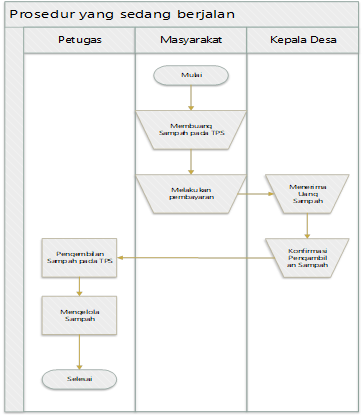
\includegraphics[width=8cm]{figures/analisis/1.png}
		\centering
		\caption{Gambar Prosedur yang sedang berjalan}
	\end{figure}
Keterangan :
\begin{enumerate}
	\item Masyarakat membuang sampah pada TPS yang sudah tersedia di depan rumahnya masing-masing
	\item Masyarakat Melakukan pembayaran ke kepala desa setiap sebulan sekali
	\item Kepala desa mengkonfirmasi ke pada petugas kebersihan untuk melakukan pengambilan sampah setiap seminggu 2 kali.
	\item Petugas kebersiahan akan mengambil sampah setiap 2 kali dalam seminggu.
	\item Petugas kebersiahan akan mengelola sampah, sampah apa saja yang akan di daur ulang dan sampah apa saja yang akan di bakar.
\end{enumerate}

\subsubsection{Analisis Sistem yang akan di bangun}
\hfill\\
Pada analisis sistem yang akan dibangun ini, dibuat beberpa pembaruan dari yang  sebelumnya. Pada prosedur ini masyarakat di haruskan mendaftarkan terlebih dahulu untuk menjadi nasabah pada Bank Sampah. Prosedur yang akan dibangun pada Bank Sampah yaitu sebagai berikut :
	\begin{figure}[H]
		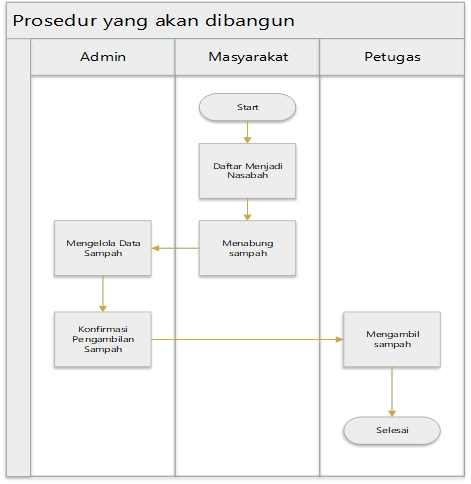
\includegraphics[width=8cm]{figures/analisis/2.png}
		\centering
		\caption{Gambar Prosedur yang akan berjalan}
	\end{figure}
Keterangan :
\begin{enumerate}
	\item Masyarakat harus mendaftarkan diri terlebih dahulu untuk menjadi nasabah pada bank sampah
	\item Setelah menjadi nasabah, masyarakat dapat menabung sampah pada bank sampah
	\item Jika masyarakat menabung sampah, maka data-data sampah tersebut akan di kelola oleh admin 
	\item Admin akan mengkonfirmasi kepada petugas untuk melakukan pengambilan sampah pada nasabah yang telah menabung sampah
	\item Petugas akan diberi alamat nasabah oleh admin
	\item Petugas melakukan pengambilan sampah ke alamat nasabah
\end{enumerate}

\subsubsection{Analisis Sistem Login yang akan di bangun}
\hfill\\
Pada analisis sistem yang akan dibangun ini, dibuat beberpa pembaruan dari yang  sebelumnya. Pada prosedur ini masyarakat di haruskan mendaftarkan terlebih dahulu untuk menjadi nasabah pada Bank Sampah. Prosedur login yang akan dibangun pada Bank Sampah yaitu sebagai berikut :
	\begin{figure}[H]
		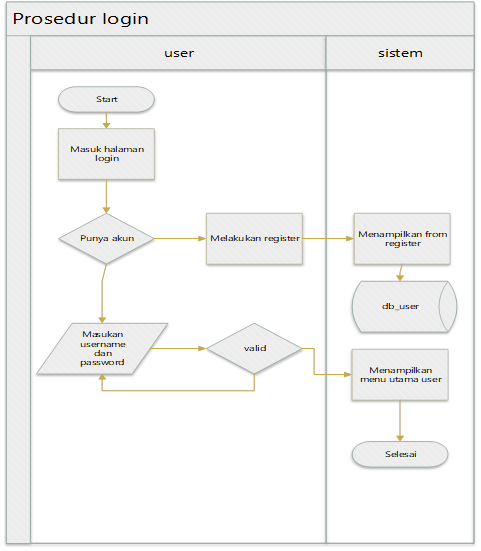
\includegraphics[width=8cm]{figures/analisis/3.png}
		\centering
		\caption{Gambar Prosedur login}
	\end{figure}
	
\begin{itemize}
\item Kebutuhan Fungsional (Functional Requirements)
\hfill\\
Kebutuhan fungsional adalah jenis kebutuhan yang berisi proses-proses apa saja yang nantinya dilakukan oleh sistem. Kebutuhan fungsional juga berisi informasi-informasi apa saja yang harus ada dan dihasilkan oleh sistem.
Adapun kebutuhan fungsional yang akan dibuat yaitu:
	\begin{enumerate}
		\item Login
		\item Kelola data user
		\item Kelola data sampah
		\item Menabung sampah
		\item Pengambilan sampah
	\end{enumerate}
Setiap proses memiliki respresentasi masing-masing pada sebuah tabel atau data yang terdapat pada database yang telah dirancang sebelumnya. Dan setiap proses berhubungan langsung dengan entitas atau user.

\item Kebuthan Non-Fungsional (Non-Functional Requirement)
Analisis kebutuhan non fungsional dilakukan untuk mengetahui spesifikasi kebutuhan untuk sistem. Spesifikasi kebutuhan melibatkan analisis perangkat keras/hardware, analisis perangkat lunak/software, analisis pengguna/user.
Adapun kebutuhan non fungsional yang akan dibuat adalah sebagai berikut :
	
	\begin{enumerate}
		\item Kebutuhan Perangkat Keras
		\hfill\\
		Pembuatan aplikasi ini menggunakan perangkat sebagai berikut :
\begin{table}[H]
\caption{Kebutuhan perangkat keras}
\centering
\begin{tabular}{c c c}
\hline \hline
No. & Jenis & Keterangan \\ [0.5ex]
\hline
1 & Processor & Inter Core i3 \\
2 & Memory & 4GB \\
3 & Monitor & LCD 14,1 Inchi \\
4 & Mouse dan keyboard & Standard \\ [1ex]
\hline
\end{tabular}
\label{tabel:nonlin}
\end{table}				
		
		\item Kebutuhan Perangkat Lunak
		\hfill\\
		Spesifikasi perangkat lunak yang digunakan adalah sebagai berikut :
\begin{table}[H]
\caption{Kebutuhan perangkat lunak}
\centering
\begin{tabular}{c c c}
\hline \hline
No. & Jenis & Keterangan \\ [0.5ex]
\hline
1 & Sistem operasi & Windows 10 Pro 64-bit \\
2 & Server database & XAMPP 1.8.1 \\
3 & Bahasa pemrogramman & PHP dan Android \\
4 & Software pendukung & Visual Studio Code dan Android Studio \\ 
5 & Browser & Chrome \\ [1ex]
\hline
\end{tabular}
\label{tabel:nonlin}
\end{table}
		
		\item Analisis Pengguna/User
		\hfill\\
		Aplikasi yang akan dibuat ini digunakan ketika ingin menabung sampah dan melakukan penjemputan sampah, adapun User yang dilibatkan antara lain : Nasabah (Masyarakat) dan petugas kebersihan.
	\end{enumerate}
\end{itemize}

\subsection{Perancangan}
\subsubsection{Usecase Diagram}
\hfill\\
Use case diagram mendeskripsikan sebuah interaksi antara satu atau lebih actor dengan sistem informasi yang akan dibuat. Use case diagram digunakan untuk mengetahui fungsi apa saja yang ada di dalam sebuah sistem informasi dan siapa saja yang berhak menggunakan fungsi-fungi itu.
	\begin{figure}[H]
		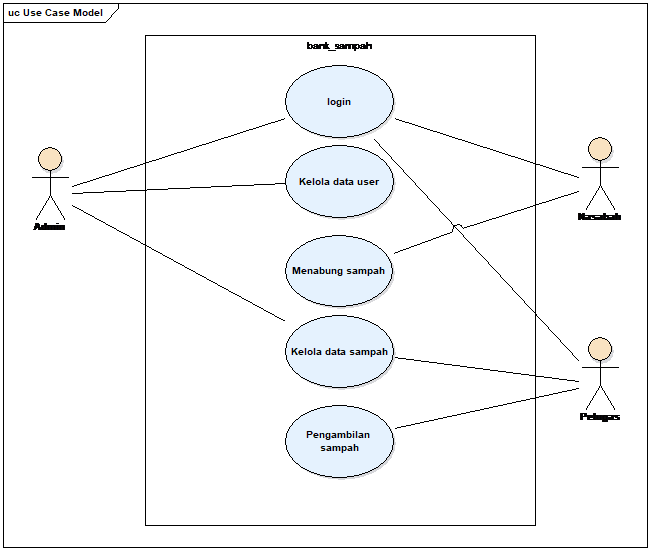
\includegraphics[width=8cm]{figures/analisis/4.png}
		\centering
		\caption{Gambar Usecase diagram}
	\end{figure}
\begin{enumerate}
\item Definisi Aktor
\hfill\\
Pada bagian ini akan dideskripsikan actor-aktor yang terlibat dalam Aplikasi Bank Sampah.
\begin{table}[H]
\caption{Definisi aktor}
\centering
\begin{tabular}{c c c}
\hline \hline
No & Aktor   & Deskripsi \\
1. & Admin   & \begin{tabular}[c]{@{}l@{}}- Mengelola data sampah\\   - Mengelola data user\\   - Mengatur jadwal pengambilan sampah\end{tabular} \\
2. & Nasabah & - Menabung sampah \\
3. & Petugas & - Kelola data sampah \\
\hline
\end{tabular}
\end{table}

\item Definisi Usecase
\hfill\\
Use case digunakan untuk mengetahui fungsi apa aja yang ada didalam sebuah sistem informasi dan siapa saja yang berhak menggunakan fungsi-fungsi itu.
\begin{table}[H]
\caption{Definisi usecase}
\centering
\begin{tabular}{lll}
\hline \hline
No  & Use Case           & Deskripsi \\
1.  & Login              & \begin{tabular}[c]{@{}l@{}}Merupakan aktifitas validasi user yang bisa \\ melakukan akses data kedalam sistem.\end{tabular} \\
2.  & Kelola data user   & Merupakan  aktifitas untuk mengelola data sampah,                                \\
3.   & Kelola data sampah & Merupakan aktifitas untuk mengelola data nasabah.                                \\
4.   & Menabung sampah    & \begin{tabular}[c]{@{}l@{}}Merupakan aktifitas untuk meminta jadwal \\ pengambilan sampah pada admin\end{tabular}           \\
5. & Pengambilan sampah & Merupakan aktifitas untuk melakukan pengambilan sampah. \\
\hline
\end{tabular}
\end{table}

\item Skenario Usecase 
\hfill\\
Skenario Usecase mendeskripsikan urutan langkah-langkah dalam proses bisnis, baik yang dilakukan aktor terhadap sistem maupun yang dilakukan oleh sistem terhadap actor.
	\begin{figure}[H]
		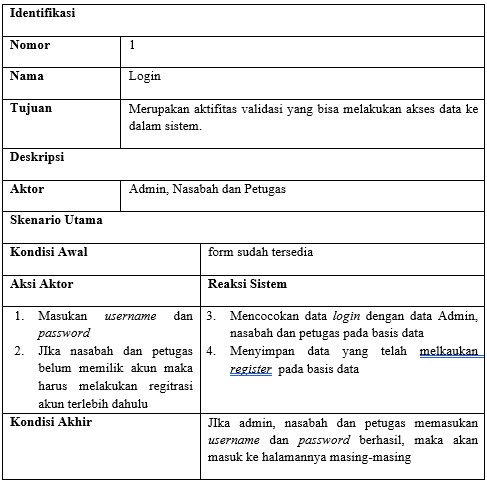
\includegraphics[width=8cm]{figures/analisis/a3.jpg}
		\centering
		\caption{Gambar Skenario Usecase}
	\end{figure}
	\begin{figure}[H]
		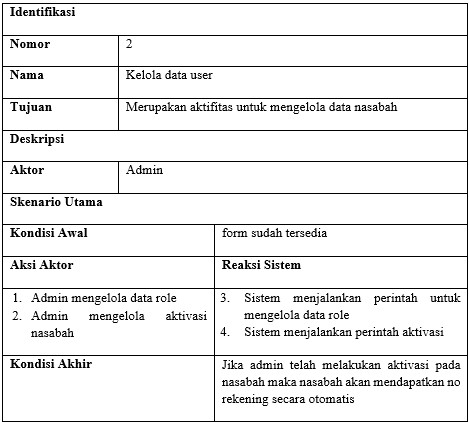
\includegraphics[width=8cm]{figures/analisis/a4.jpg}
		\centering
		\caption{Gambar Skenario Kelola data user}
	\end{figure}
	\begin{figure}[H]
		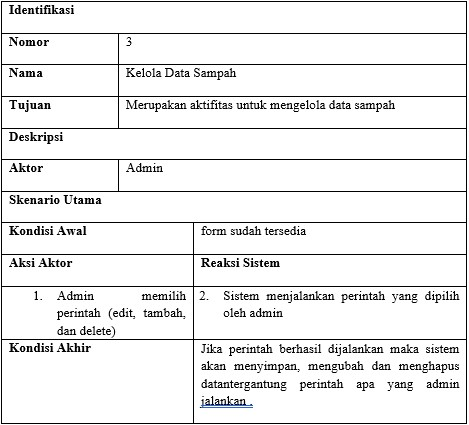
\includegraphics[width=8cm]{figures/analisis/a5.jpg}
		\centering
		\caption{Gambar Skenario Kelola sampah}
	\end{figure}	
	\begin{figure}[H]
		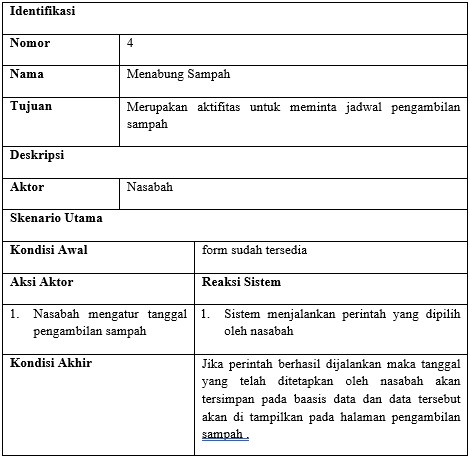
\includegraphics[width=8cm]{figures/analisis/a6.jpg}
		\centering
		\caption{Gambar Skenario menabung sampah}
	\end{figure}	
	\begin{figure}[H]
		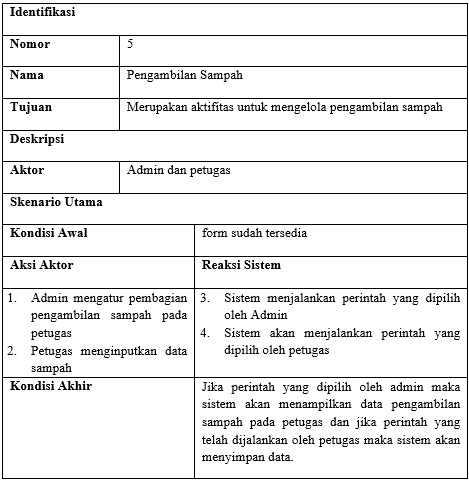
\includegraphics[width=8cm]{figures/analisis/a7.jpg}
		\centering
		\caption{Gambar Skenario pengambilan sampah}
	\end{figure}	
\end{enumerate}

\subsubsection{Class Diagram}
\hfill\\
Class diagram menggambarkan struktur sistem dari segi pendefinisian kelas – kelas yang akan dibuat untuk membangun sistem.
	\begin{figure}[H]
		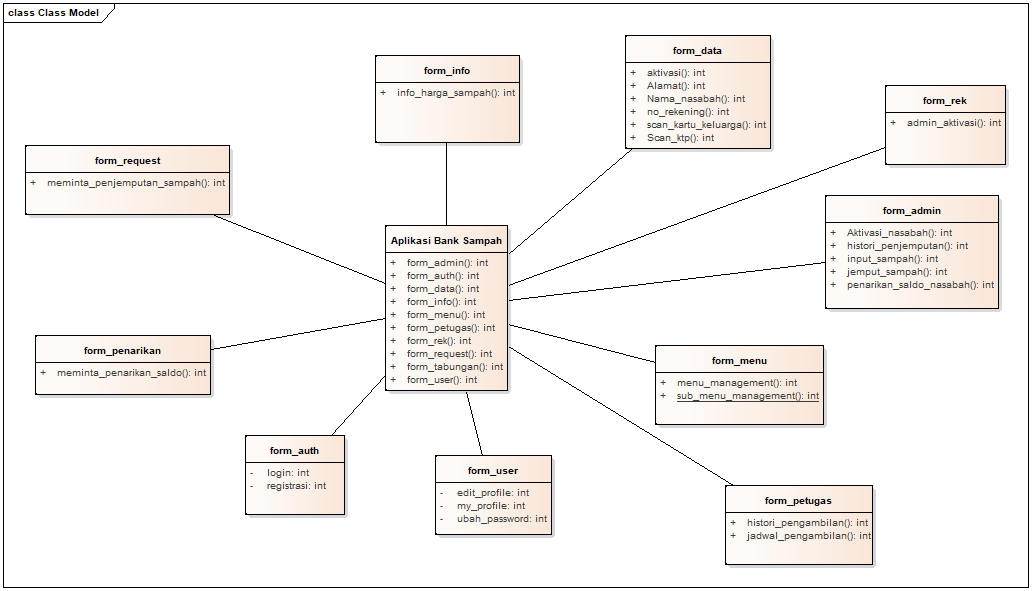
\includegraphics[width=8cm]{figures/analisis/5.png}
		\centering
		\caption{Gambar Class Diagram}
	\end{figure}
	
\subsubsection{Sequence Diagram}
\hfill\\
Squence diagram menggambarkan kelakuan objek pada use case dengan mendeskripsikan waktu hidup objek dan pesan yang dikirimkan dan diterima antar objek.
\begin{enumerate}
\item Squence Diagram Login
\hfill\\
	\begin{figure}[H]
		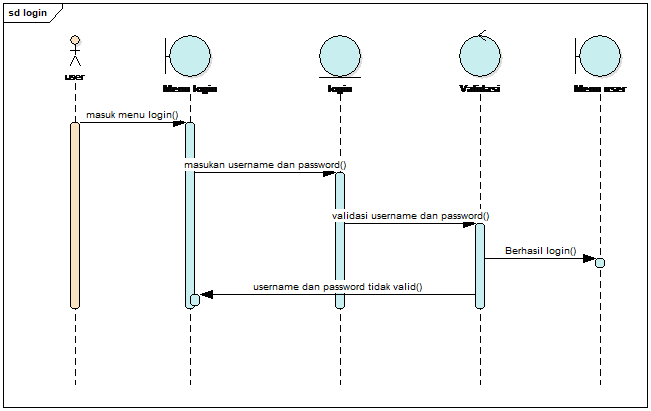
\includegraphics[width=8cm]{figures/analisis/6.png}
		\centering
		\caption{Gambar Sequence Diagram Kelola Login}
	\end{figure}
\textbf{Deskripsi Sequence Login :}
\hfill\\
Pada Sequence Diagram ini menjelaskan proses login. Admin, nasabah, dan petugas mulai memasukkan username dan password pada menu login. Kemudian database akan mengecek validasi, jika username dan password benar maka akan masuk ke sistem dan tampil halaman awal sistem. Jika username dan password salah maka kembali memasukkan username dan password.

\item Sequence Diagram Kelola User
\hfill\\
	\begin{figure}[H]
		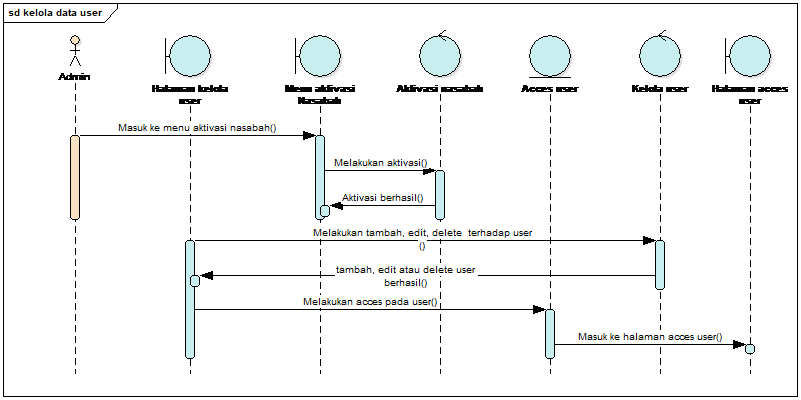
\includegraphics[width=8cm]{figures/analisis/7.png}
		\centering
		\caption{Gambar Sequence Diagram Kelola User}
	\end{figure}
\textbf{Deskripsi Sequence User :}
\hfill\\
Pada Sequence Diagram ini menjelaskan admni yang melakukan proses pengelolaan data nasabah memilih menu aktivasi nasabah lalu sistem akan memproses dan memberikan no.rekening kepada nasabah. Selanjutnya nasabah akan mendapatkan no.rekening dan dapat melakukan proses menabung sampah pada Aplikasi Bank Sampah.

\item Sequence Diagram Menabung Sampah
\hfill\\
	\begin{figure}[H]
		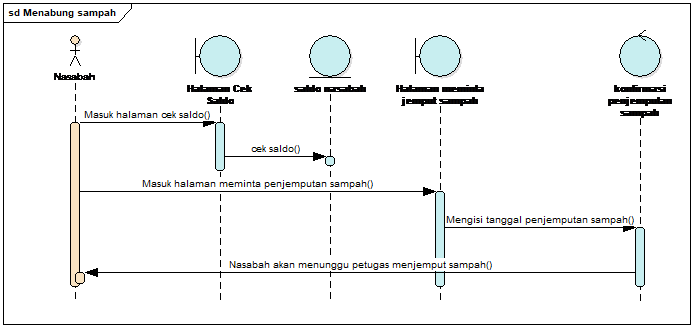
\includegraphics[width=8cm]{figures/analisis/8.png}
		\centering
		\caption{Gambar Sequence Menabung Sampah}
	\end{figure}
\textbf{Deskripsi Sequence Menabung Sampah :}
\hfill\\
Pada Sequence Diagram ini menjelaskan proses menabung sampah yang dilakukan oleh nasabah, disini nasabah akan mengatur tanggal untuk pengambilan sampah, maka sistem akan menyimpan tanggal tersebut dan akan di tampilkan pada halaman admin di menu jadwal pengambilan sampah. 

\item Sequence Diagram Kelola Data Sampah
\hfill\\
	\begin{figure}[H]
		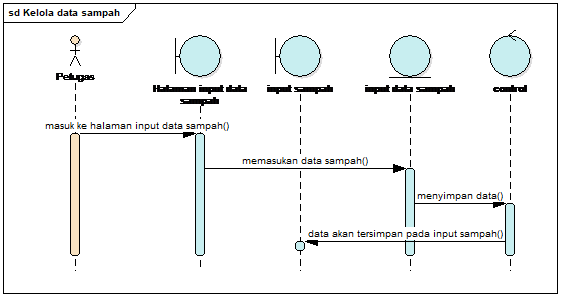
\includegraphics[width=8cm]{figures/analisis/9.png}
		\centering
		\caption{Gambar Sequence Diagram Kelola Data Sampah}
	\end{figure}
\textbf{Deskripsi Sequence Data Sampah :}
\hfill\\
Deskripsi Squence Kelola Data Sampah :
Pada Sequence Diagram ini menjelaskan proses penginputan data sampah oleh petugas kebersihan setelah melakukan pengambilan sampah pada nasabah, sistem akan menyimpan data yang telah di inputkan oleh petugas. 

\item Sequence Diagram Pengambilan Sampah
\hfill\\
	\begin{figure}[H]
		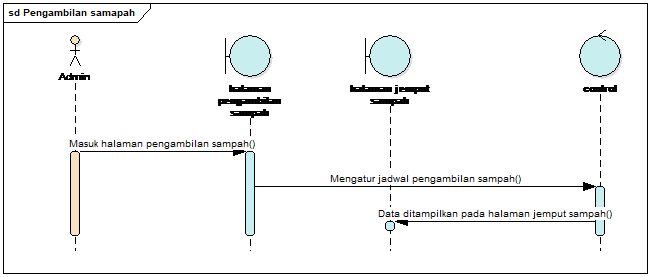
\includegraphics[width=8cm]{figures/analisis/10.png}
		\centering
		\caption{Gambar Sequence Diagram Pengambilan Sampah}
	\end{figure}
\textbf{Deskripsi Sequence Pengambilan Sampah :}
\hfill\\
Pada Sequence Diagram ini menjelaskan proses pengambilan sampah yang akan di atur oleh admin, disni admin akan mengatur petugas mana yang akan melakukan pengambilan sampah pada nasabah. Sistem akan menyimpan data penjemputan sampah dengan status diambil dan belum diambil.

\end{enumerate}

\subsubsection{Activity Diagram}
Activity Diagram adalah sebuah diagram alur kerja yang menjelaskan berbagai kegiatan pengguna (atau sistem), orang yang melakukan masing-masing aktivitas, dan aliran sekuensial dari aktivitas-aktivitas tersebut.
\begin{enumerate}

\item Activity Diagram Login
\hfill\\
	\begin{figure}[H]
		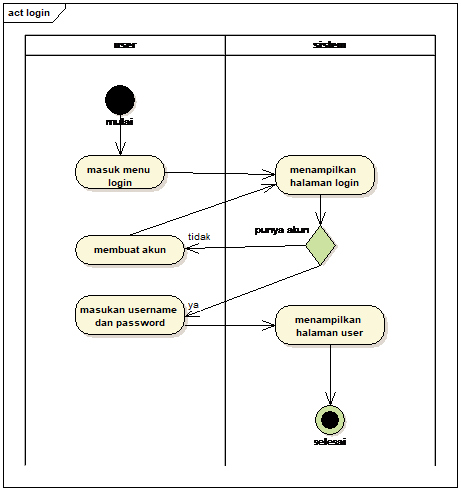
\includegraphics[width=8cm]{figures/analisis/11.png}
		\centering
		\caption{Gambar Activity Diagram Kelola Login}
	\end{figure}
\textbf{Deskripsi Activity Diagram Login:}
\hfill\\
Pada Activity Diagram ini menjelaskan tentang proses login. Dimulai dari admin, pemilik dan peminjam menginput username dan password, kemudian sistem akan memvalidasi user. Jika valid maka sistem akan menampilkan menu utama. Jika tidak valid, maka admin, pemilik dan peminjam kembali menginput username dan password.	
	
\item Activity Diagram Login
\hfill\\
	\begin{figure}[H]
		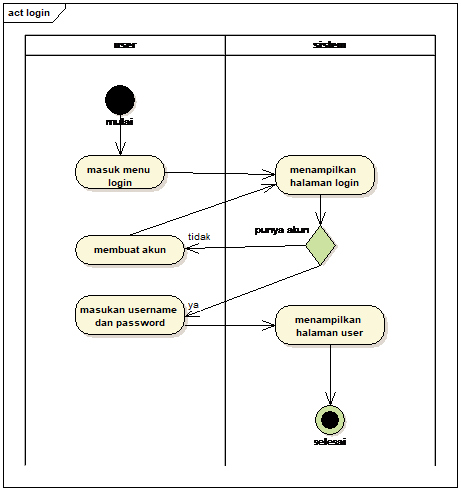
\includegraphics[width=8cm]{figures/analisis/11.png}
		\centering
		\caption{Gambar Activity Diagram Kelola Login}
	\end{figure}
\textbf{Deskripsi Activity Diagram Login:}
\hfill\\
Pada Activity Diagram ini menjelaskan tentang proses login. Dimulai dari admin, pemilik dan peminjam menginput username dan password, kemudian sistem akan memvalidasi user. Jika valid maka sistem akan menampilkan menu utama. Jika tidak valid, maka admin, pemilik dan peminjam kembali menginput username dan password.	
	
\item Activity Diagram Kelola Data User
\hfill\\
	\begin{figure}[H]
		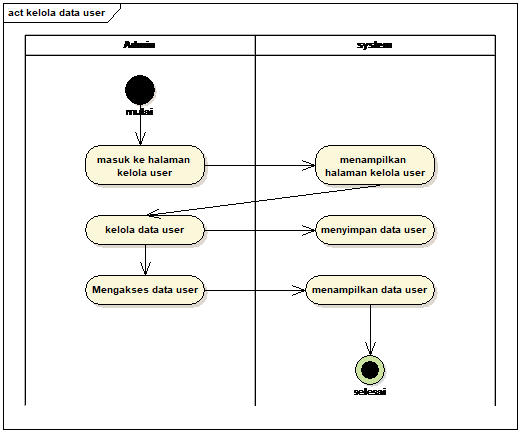
\includegraphics[width=8cm]{figures/analisis/12.png}
		\centering
		\caption{Gambar Activity Diagram Kelola Data User}
	\end{figure}
\textbf{Deskripsi Activity Diagram Kelola Data User:}
\hfill\\
Pada Activity Diagram ini menjelaskan admni yang melakukan proses pengelolaan data nasabah memilih menu aktivasi nasabah lalu sistem akan memproses dan memberikan no.rekening kepada nasabah. Selanjutnya nasabah akan mendapatkan no.rekening dan dapat melakukan proses menabung sampah pada Aplikasi Bank Sampah.
	
\item Activity Diagram Kelola Data Sampah
\hfill\\
	\begin{figure}[H]
		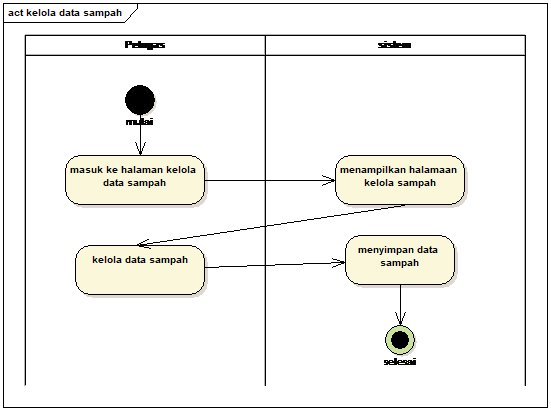
\includegraphics[width=8cm]{figures/analisis/14.png}
		\centering
		\caption{Gambar Activity Diagram Menabung Sampah}
	\end{figure}
\textbf{Deskripsi Activity Diagram Kelola Data Sampah:}
\hfill\\
Pada Activity Diagram ini menjelaskan proses penginputan data sampah oleh petugas kebersihan setelah melakukan pengambilan sampah pada nasabah, sistem akan menyimpan data yang telah di inputkan oleh petugas. 
	
\item Activity Diagram Pengambilan Sampah
\hfill\\
	\begin{figure}[H]
		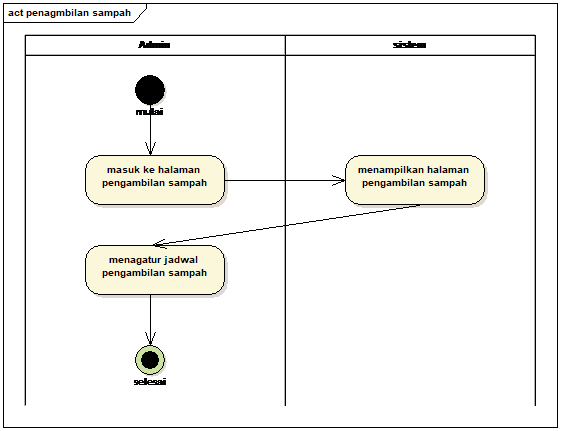
\includegraphics[width=8cm]{figures/analisis/15.png}
		\centering
		\caption{Gambar Activity Diagram Pengambilan Sampah}
	\end{figure}
\textbf{Deskripsi Activity Diagram Pengambilan Sampah:}
\hfill\\
Pada Sequence Diagram ini menjelaskan proses pengambilan sampah yang akan di atur oleh admin, disni admin akan mengatur petugas mana yang akan melakukan pengambilan sampah pada nasabah. Sistem akan menyimpan data penjemputan sampah dengan status diambil dan belum diambil.
	
\end{enumerate}

\subsubsection{Deployment Diagram}
	\begin{figure}[H]
		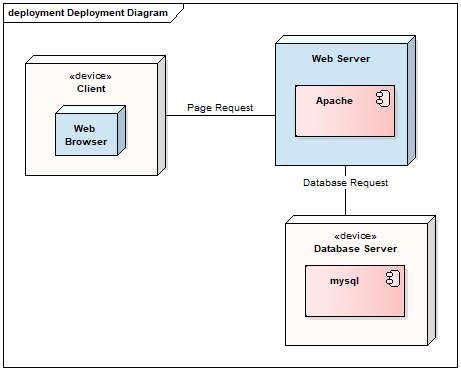
\includegraphics[width=8cm]{figures/analisis/16.png}
		\centering
		\caption{Gambar Deployment Diagram}
	\end{figure}
	\textbf{Deskripsi Deployment Diagram :}
\hfill\\
Pada Deployment diagram ini menggambarkan arsitektur perangkat secara fisik yang membentuk sistem informasi yang akan dibangun. Untuk aplikasi atau sistem yang berbasis web dibentuk oleh komponen hardware dan software yang saling berkaitan.

\subsubsection{Struktur Diagram}
	\begin{figure}[H]
		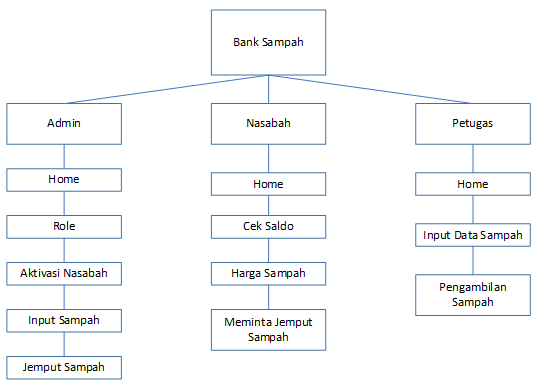
\includegraphics[width=8cm]{figures/analisis/17.png}
		\centering
		\caption{Gambar Struktur Diagram}
	\end{figure}
	\textbf{Deskripsi Struktur Diagram :}
\hfill\\
Pada Struktur Diagram Menu ini menjelaskan struktur menu yang ada pada aplikasi bank sampah, mulai dari admin, user dan petugas masuk ke menu login akan masuk ke menu yang sudah ditentukan. Sehingga mereka hanya dapat mengakses menu-menu yang muncul ketika mereka login.

\section{Tampilan User Interface}
\subsubsection{Tampilan Page Registrasi}
\hfill\\
	\begin{figure}[H]
		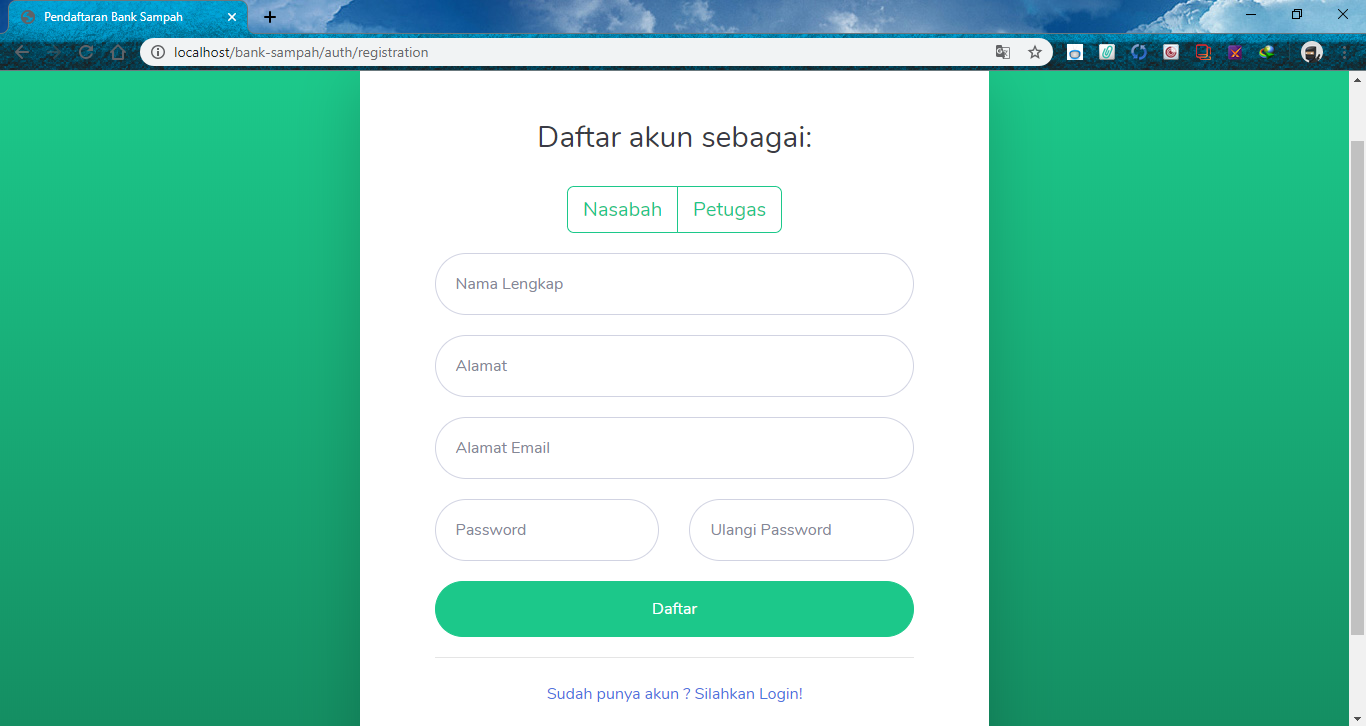
\includegraphics[width=8cm]{figures/analisis/18.png}
		\centering
		\caption{Gambar Page Registrasi}
	\end{figure}
Penjelasannya:
\begin{enumerate}
\item Dimulai dari page registrasi, masyarakat yang akan mendaftarkan diri sebagai nasabah atau petugas memulai dengan melakukan proses registrasi terlebih dahulu agar nasabah ataupun petugas dapat memiliki akun dan memudahkan admin dalam melakukan pengelolaan user. Pada halaman registrasi ini masyarakat harus melengkapi from registrasi dan memilih akan mendaftar sebagai nasabah atau sebagai petugas. Setelah from registrasi telah dilengkapi dengan  benar dan sesuai. 
\item Setelah form registrasi telah di isi dengan benar dan sesuai maka klik tombol button daftar agar dapat mendapatkan akun, sehingga dapat melakukan proses login.
\end{enumerate}

\subsubsection{Tampilan Page Login}
\hfill\\
	\begin{figure}[H]
		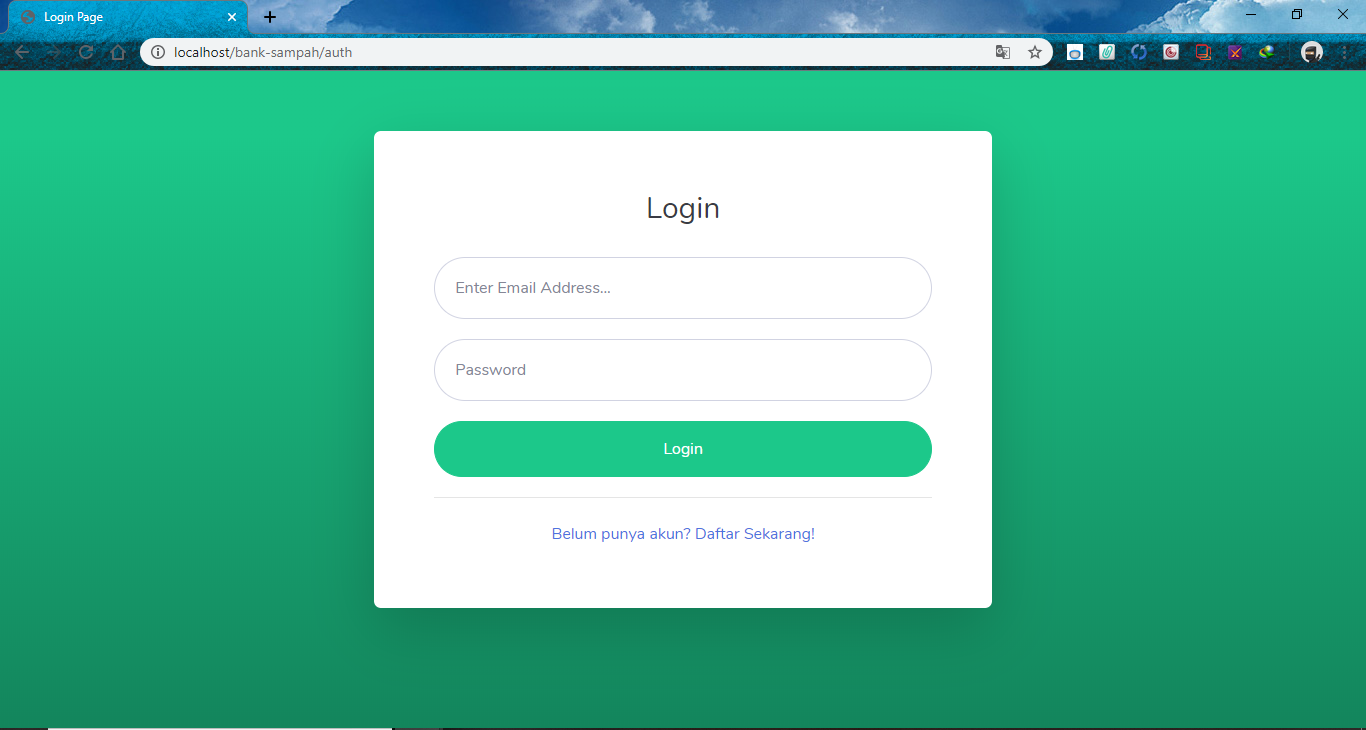
\includegraphics[width=8cm]{figures/analisis/19.png}
		\centering
		\caption{Gambar Page Login}
	\end{figure}
Penjelasannya :
\begin{enumerate}
\item Ketika masyarakat telah melakukan proses registrasi sebagai nasabah atau sebagai petugas maka masyarakat dapat melakukan proses login. Pada halaman login ini admin, nasabah dan petugas dapat melakukan proses login. Ketika user (admin, nasabah dan petugas) menginputkan alamat email dan password dengan benar, maka user akan masuk ke halaman yang telah ditentukan. Jika alamat email dan passwordnya tidak valid maka user diharuskan menginput ulang alamat email dan password dengan benar. 
\item Klik tombol login agar dapat masuk ke halaman utama user (admin, nasabah dan petugas).
\end{enumerate}

\subsection{Tampilam Admin}

\subsubsection{Tampilan Page Role}
\hfill\\
	\begin{figure}[H]
		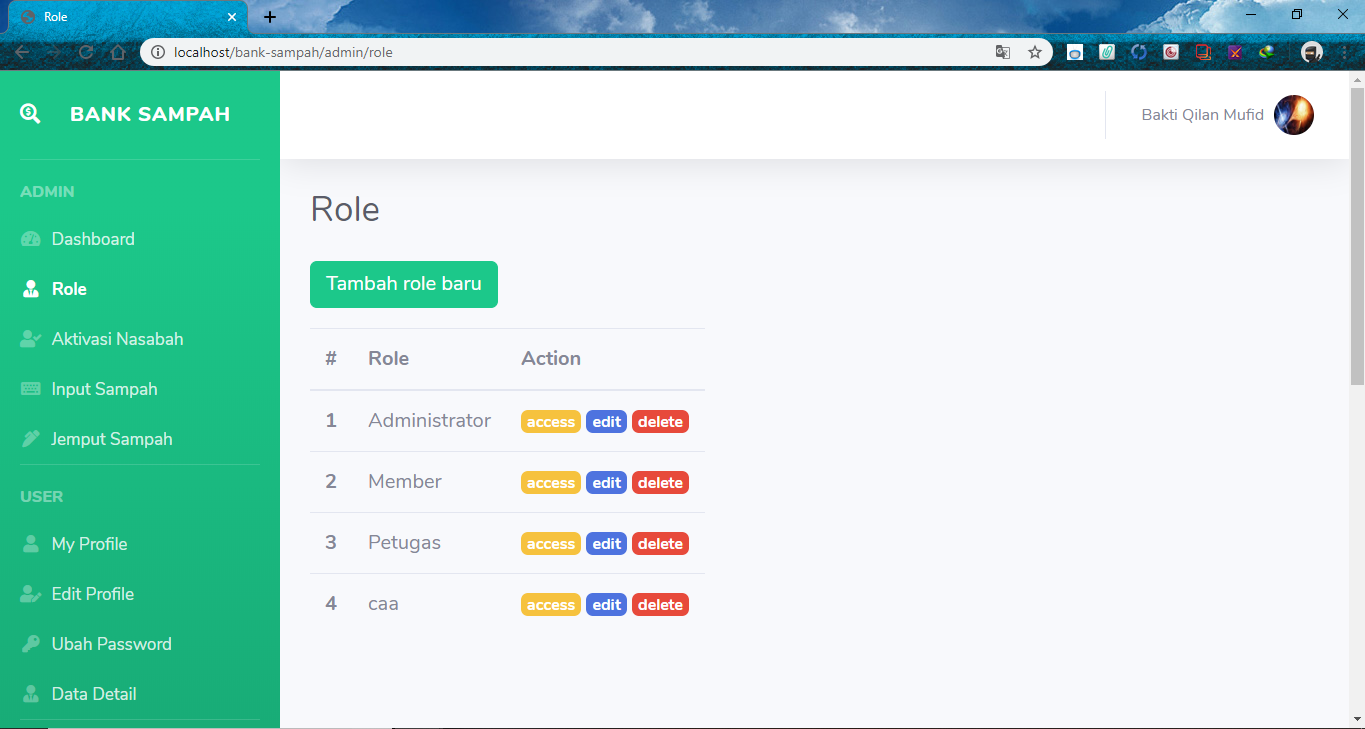
\includegraphics[width=8cm]{figures/analisis/20.png}
		\centering
		\caption{Gambar Page Role}
	\end{figure}
Penjelasannnya :
\begin{enumerate}
\item Tampilan page role merupakan halaman awal ketika admin berhasil melakukan proses login, pada halaman ini admin dapat melakukan proses tambah, acces, edit dan delete role sesuai apa yang diinginkan oleh admin.  
\item Tombol button tambah untuk menambahkan role baru.
\item Tombol button acces untuk mengakses role tersebut.
\item Tombol button edit untuk mengatur atau memperbaiki jika role tersebut ada kesalahan
\item Tombol button delete untuk menghapus role lama atau jika ada kesalahan dalam menambahkan role baru.
\end{enumerate}

	
\subsubsection{Tampilan Page Aktivasi Nasabah}
\hfill\\
	\begin{figure}[H]
		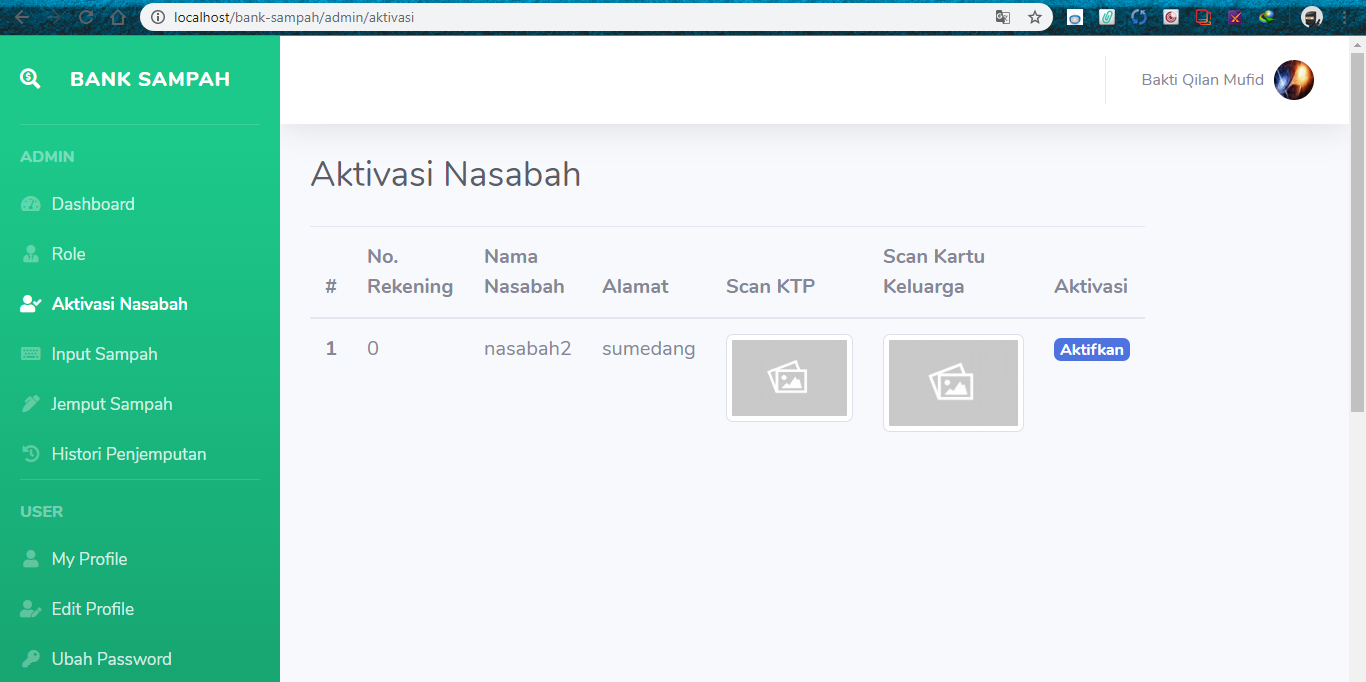
\includegraphics[width=8cm]{figures/analisis/21.png}
		\centering
		\caption{Gambar Page Aktivasi Nasabah}
	\end{figure}
Penjelasannya :
\begin{enumerate}
\item Ketika nasabah telah melakukan proses registrasi dan melengkapi persyaratan yang berlaku pada bank sampah ini maka admin dapat melakukan proses aktivasi nasbaah. Ketika admin telah melakukan proses aktivasi maka akun nasabah tersebut akan mendapatkan no.rekening sehingga dapat memulai melakukan proses menabung sampah. 
\item Tombol button aktivasi untuk melakukan proses aktivasi admin terhadap nasabah baru yang telah menyelesaikan proses registrasi dan telah melengkapi persyaratan.
\end{enumerate}
	
\subsubsection{Tampilan Page Input Sampah}
\hfill\\
	\begin{figure}[H]
		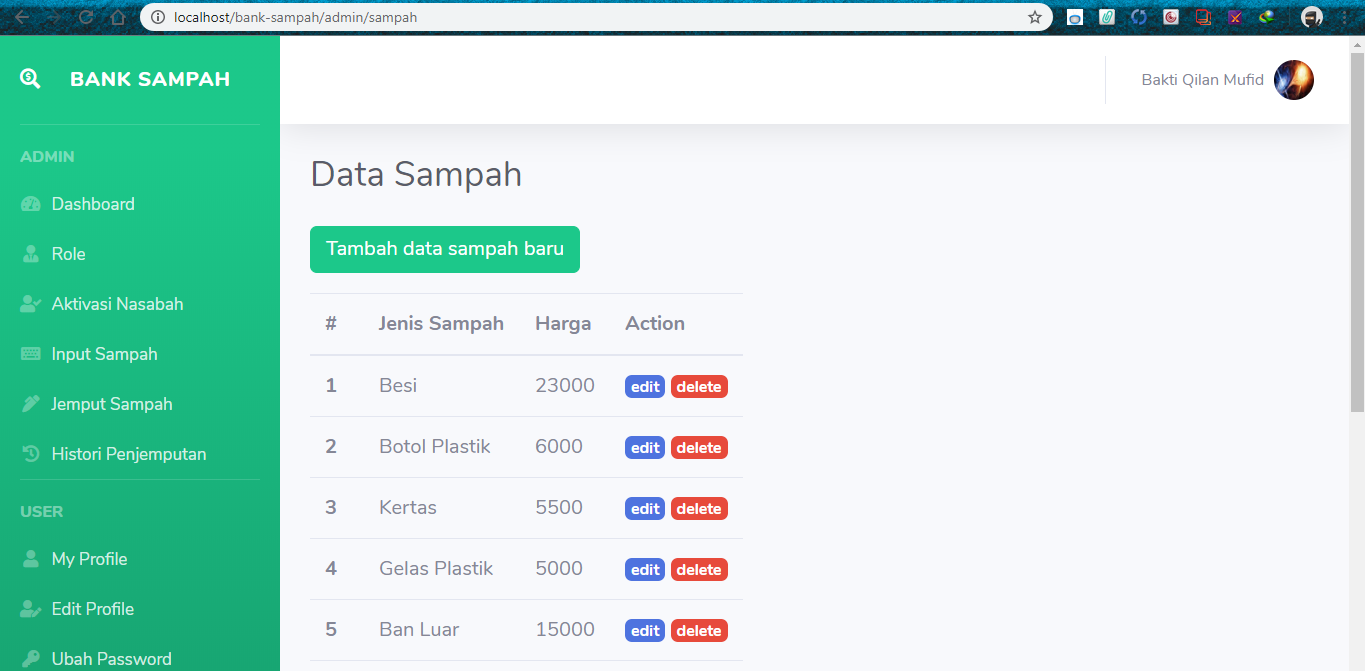
\includegraphics[width=8cm]{figures/analisis/22.png}
		\centering
		\caption{Gambar Page Input Sampah}
	\end{figure}
Penjelasannya :
\begin{enumerate}
\item Pada halaman ini admin akan melakukan proses menginputkan data-data sampah sesuai dengan harga pasarnya. Data-data yang telah admin inputkan dapat di lihat oleh nasabah dan petugas pada halaman info harga sampah. 
\item Tombol button tambah untuk menambahkan data sampah yang baru
\item Tombol button edit untuk memperbaiki data sampah jika ada kesalahan dalam proses input data sampah
\item Tombol button delete untuk menghapus data sampah jika data tersebut sudah tidak berlaku lagi.
\end{enumerate}
	

\subsubsection{Tampilan Page Jemput Sampah}
\hfill\\
	\begin{figure}[H]
		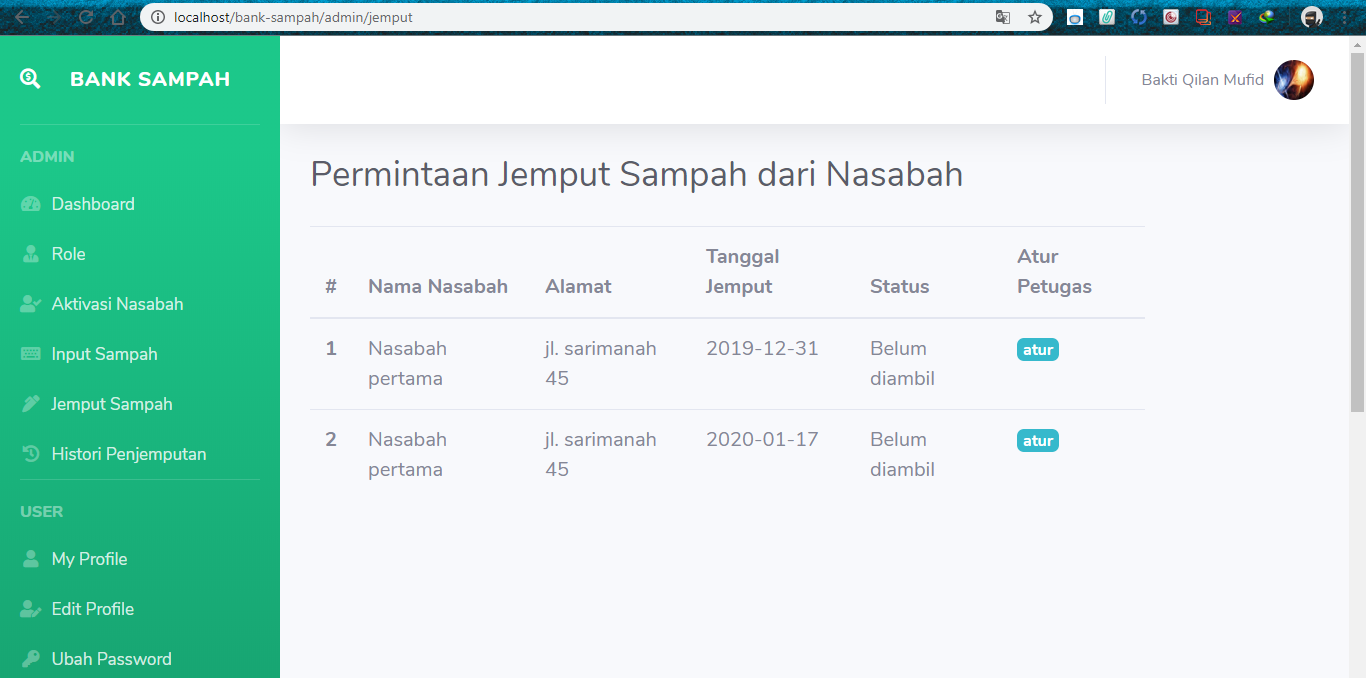
\includegraphics[width=8cm]{figures/analisis/23.png}
		\centering
		\caption{Gambar Page Jemput Sampah}
	\end{figure}
Penjelasannya :	
\begin{enumerate}
\item Admin akan mengatur petugas sampah dalam melakukan pengambilan sampah pada nasabah, sebelumnya nasabah telah menetapkan tanggal pengambilan sampahnya.Apabila proses atur berhasil maka admin akan memilih petugas ke berapa yang akan melakukan pengambilan sampah tersebut, sehingga akan masuk ke halaman pengambilan sampah ke petugas yang telah ditentukan.
\end{enumerate}
	
\subsubsection{Tampilan Page Histori Penjemputan}
\hfill\\
	\begin{figure}[H]
		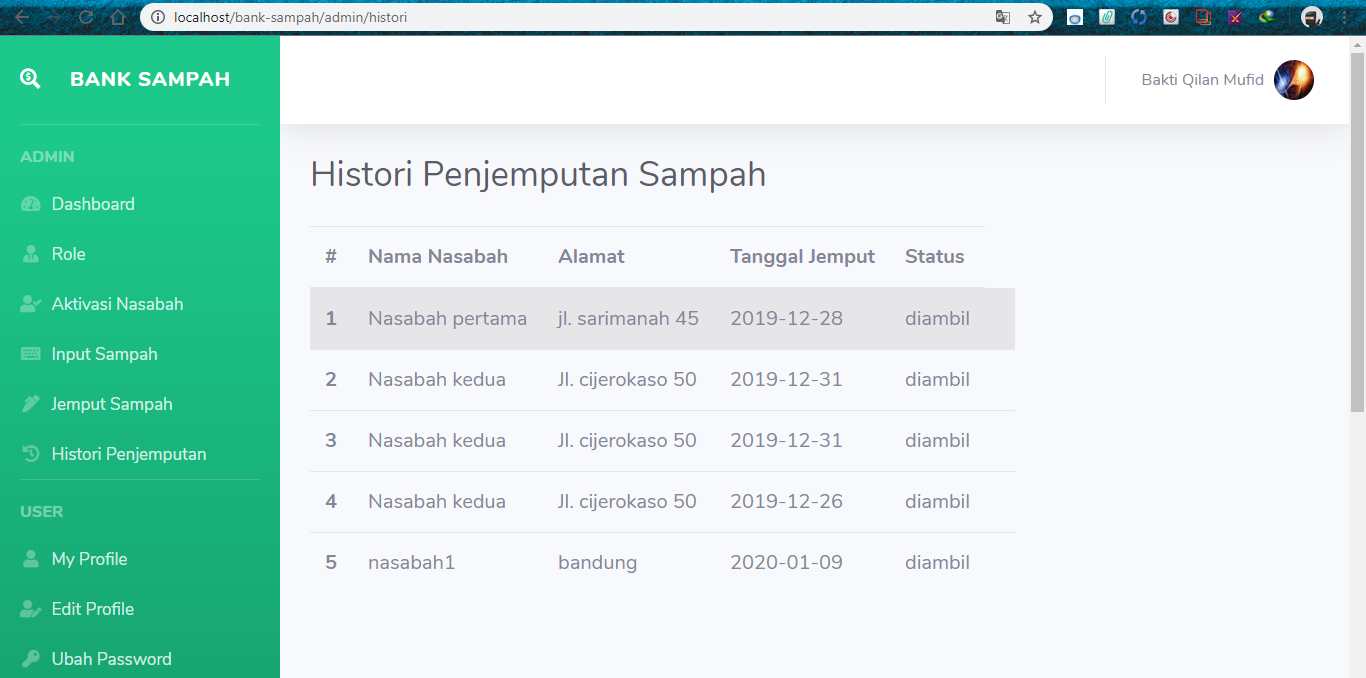
\includegraphics[width=8cm]{figures/analisis/24.png}
		\centering
		\caption{Gambar Page Histori Penjemputan}
	\end{figure}
Penjelasannya :
\begin{enumerate}
\item Pada halaman ini merupakan proses-proses penjemputan sampah yang telah diambil, sehingga memudahkan admin untuk mengontrol setiap pergerakan dari petugas kebersihan dalam menjalankan tugasnya.
\item Admin akan melihat dan mengecek menu histori penjemputan sampah.
\item Jika sampah pada nasabah telah di ambil oleh petugas maka status pada histori penjemputan sampah diambil.
\end{enumerate}

\subsubsection{Tampilan Page Menu Management}
\hfill\\
	\begin{figure}[H]
		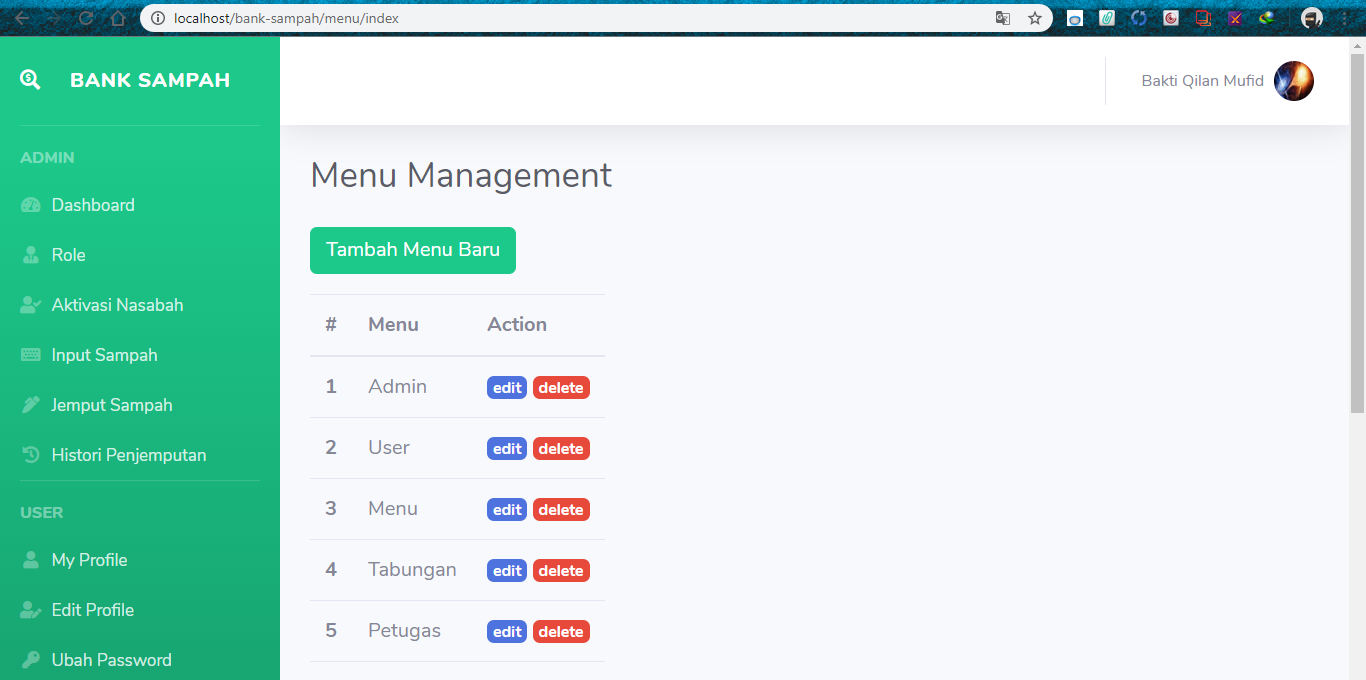
\includegraphics[width=8cm]{figures/analisis/25.png}
		\centering
		\caption{Gambar Page Menu Management}
	\end{figure}
Penjelasannya :
\begin{enumerate}
\item Pada halaman ini admin dapat menegelola data menu management, sehingga memudahkan admin jika adanya perubahan atau perbaikan terhadap aplikasi bank smapah.
\item Admin akan melakukan proses tambah, edit dan delete pada menu management.
\item Tombol button tambah untuk melakukan proses menambahkan menu management yang baru
\item Tombol button edit untuk memeperbaiki jika ada kesalahan pada menu management
\item Tombol button delete untuk menghapus data menu management jika menu tersebut sudah jarang digunakan atau tidak dibutuhkan lagi.

\end{enumerate}
	
\subsubsection{Tampilan Page Sub Menu Management}
\hfill\\
	\begin{figure}[H]
		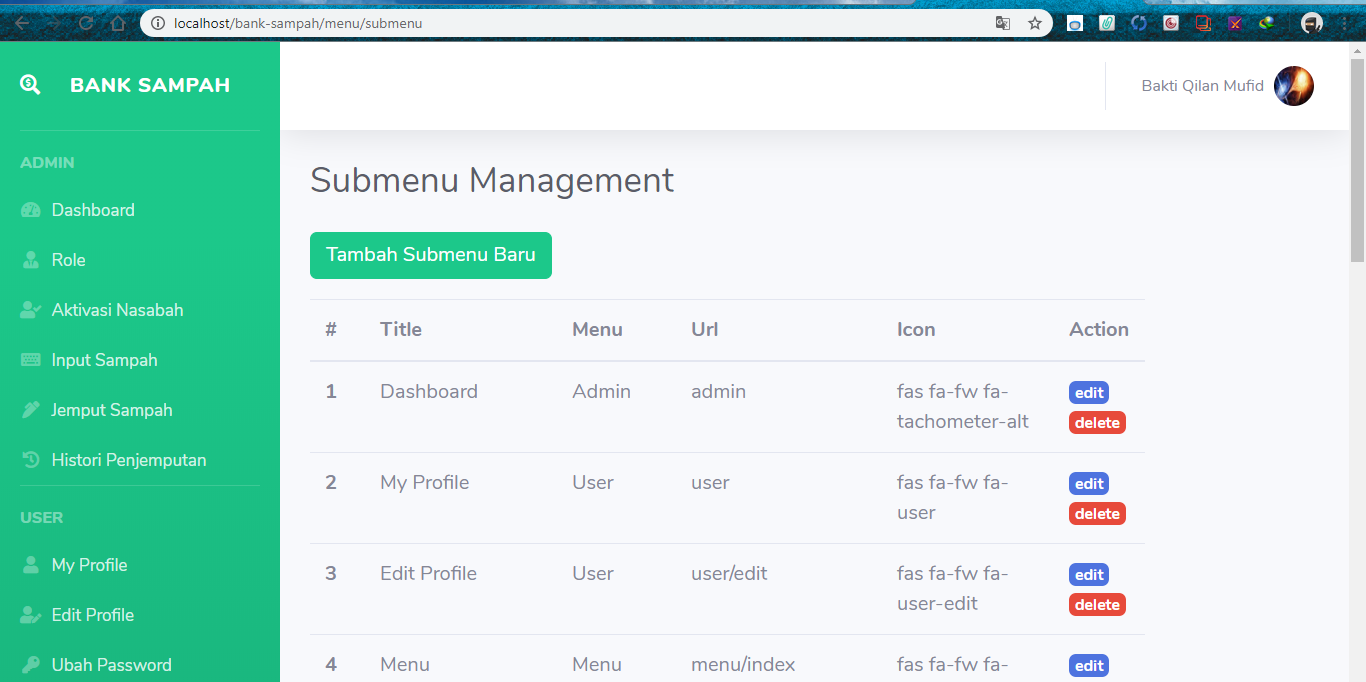
\includegraphics[width=8cm]{figures/analisis/26.png}
		\centering
		\caption{Gambar Page Sub Menu Management}
	\end{figure}
Penjelasannya :
\begin{enumerate}
\item Pada halaman ini admin dapat mengelola submenu management, sehingga memudahkan admin jika adanya perubahan atau perbaikan terhadap aplikasi bank smapah.
\item Admin akan melakukan proses tambah, edit dan delete pada sub menu management.
\item Apabila proses tambah berhasil maka akan membuat sub menu management.yang baru
\item Tombol button tambah untuk melakukan proses menambahkan menu management yang baru
\item Tombol button edit untuk memeperbaiki jika ada kesalahan pada menu management
\item Tombol button delete untuk menghapus data menu management jika menu tersebut sudah jarang digunakan atau tidak dibutuhkan lagi.
\end{enumerate}

\subsubsection{Tampilan Page Harga Sampah}
\hfill\\
	\begin{figure}[H]
		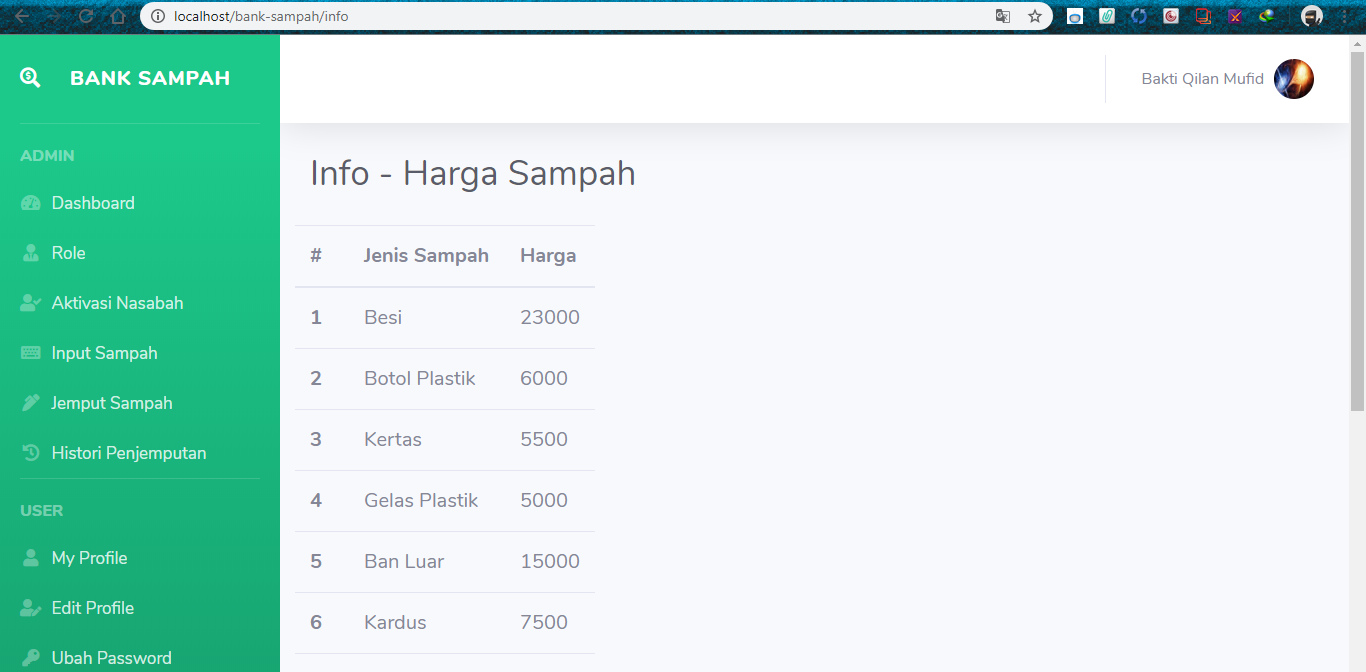
\includegraphics[width=8cm]{figures/analisis/27.png}
		\centering
		\caption{Gambar Page Harga Sampah}
	\end{figure}
Penjelasannya :
\begin{enumerate}
\item Pada halaman ini nasabah dan petugas dapat melihat atau mengecek harga-harga sampah yang dapat ditabungkan pada bank sampah, sehingga memudahkan nasabah dalam memilih sampah apa saja yang dapat ditabungkan pada bank sampah dan mempermudah petugas dalam melakukan peroses input data sampah pada nasabah yang melakukan proses menabung smapah.
\item Data-data sampah tersebut merupakan hasil dari inputan yang dikelola oleh admin pada menu input sampah 

\end{enumerate}
	

\subsection{Tampilan Nasabah}
\subsubsection{Tampilan Page Cek Saldo}
\hfill\\
	\begin{figure}[H]
		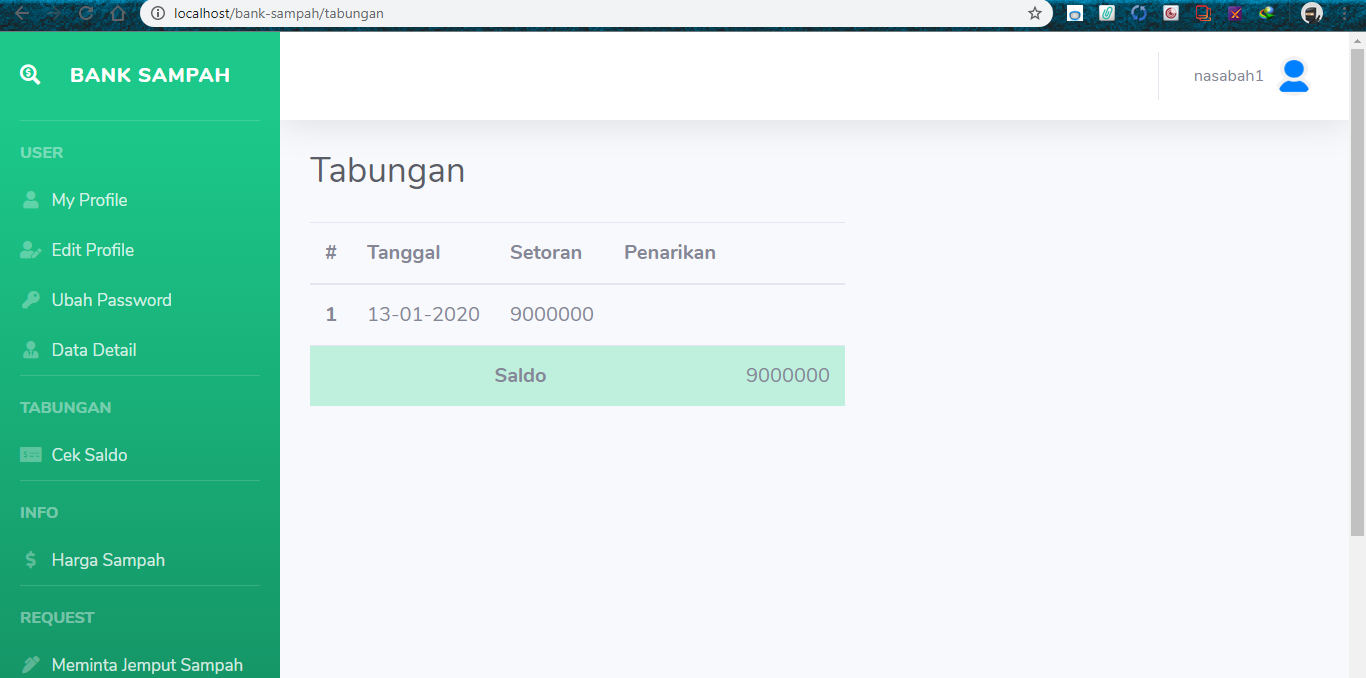
\includegraphics[width=8cm]{figures/analisis/28.png}
		\centering
		\caption{Gambar Page Cek Saldo}
	\end{figure}
Penjelasannya :
\begin{enumerate}
\item Pada halaman ini nasbah yang sudah melengkapi persyaratan dan telah diaktivasi oleh admin nasabah tersebut akan mendapatkan no.rekening dan dapat melakukukan proses menabung sampah.
\item Ketika nasabah sudah mendapatkan uang dari proses menabung sampah, maka nasabah akan mengecek uang tersebut pada halaman ini dan jika nasabah melakukan penarikan uang maka dapat melihat saldo yang tersisa pada halaman ini.
\end{enumerate}
	
\subsubsection{Tampilan Page Meminta Penjemputan Sampah}
\hfill\\
	\begin{figure}[H]
		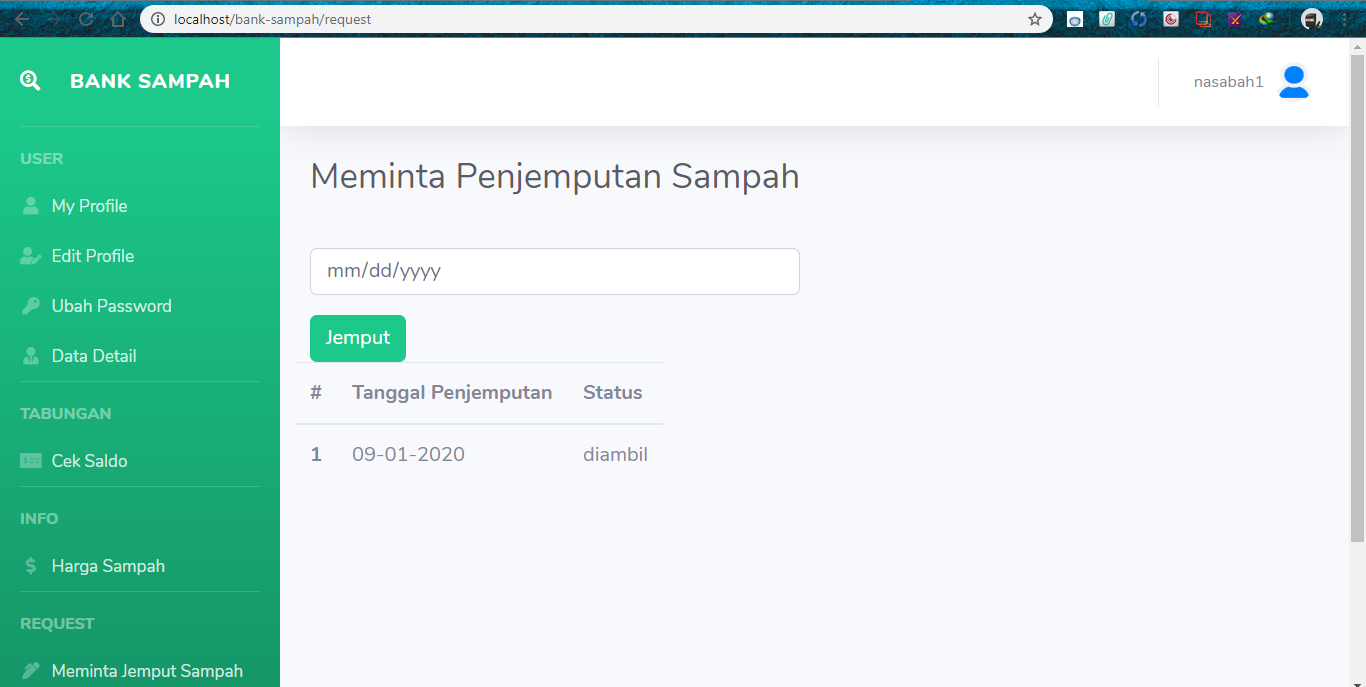
\includegraphics[width=8cm]{figures/analisis/29.png}
		\centering
		\caption{Gambar Page Meminta Penjemputan Sampah}
	\end{figure}
Penjelasannya :
\begin{enumerate}
\item Pada halaman ini nasabah dapat menentukan jadawal pengambilan sampah sesuai yang mereka inginkan, sehingga ketika nasabah telah mengatur jadwal tersebut petugas akan dating sesuai jadwal yang ditentukan oleh nasabah.
\item Tombol button jemput untuk menetapkan jadwal pengmabilan sampah
\item Ketika tombbol tersebut di klik maka akan muncul histori tanggal penjemputan sampah, sehingga nasabah dapat melihat kembali jadwal pengambilan sampah, jika sampah belum diambil maka status nya masih belum diambil dan jika sampah sudah diambil maka statusnya diambil. 
\end{enumerate}


\subsection{Tampilan Petugas}
\subsubsection{Tampilan Page Pengambilan Sampah}
\hfill\\
	\begin{figure}[H]
		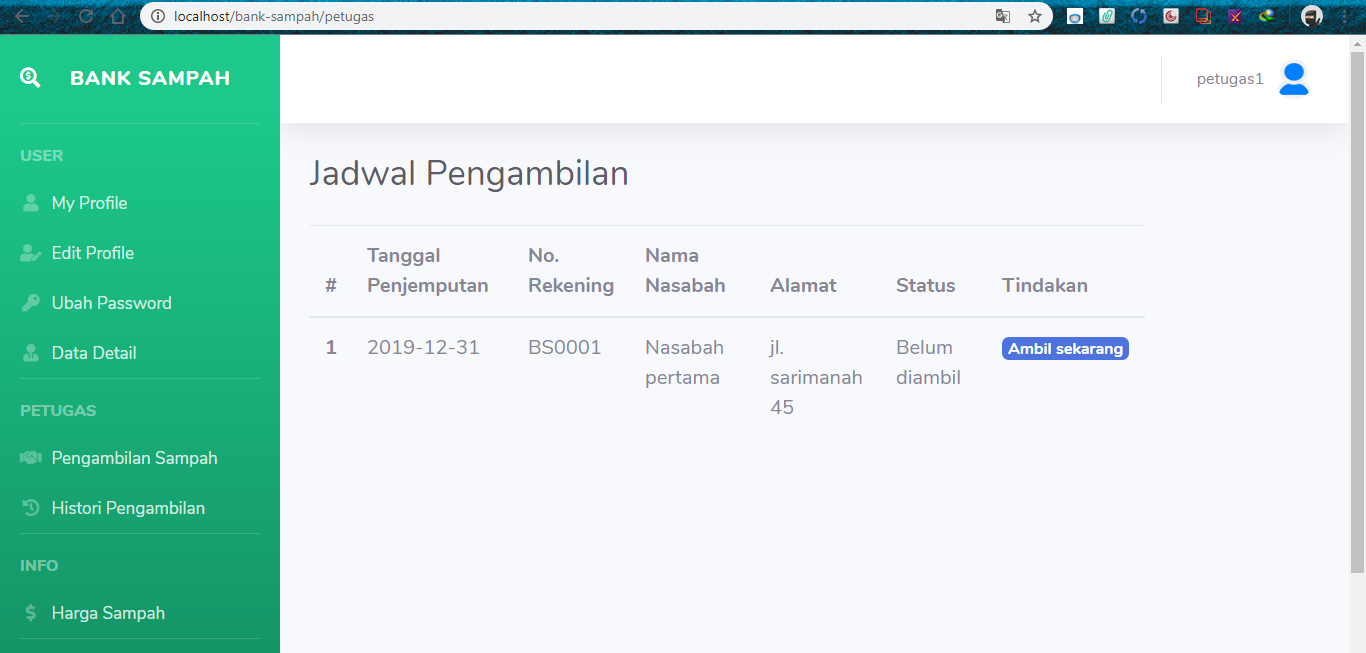
\includegraphics[width=8cm]{figures/analisis/30.png}
		\centering
		\caption{Gambar Page Pengambilan Sampah}
	\end{figure}
Penjelasannya :
\begin{enumerate}
\item Pada halaman ini Admin mengatur petugas mana yang akan melakukan pengambilan sampah jika petugas 1 yang dipilih untuk melakukan pengambilan sampah maka akan muncul pada halaman pengambilan sampah pada akun petugas 1.
\item Tombol button ambil sekarang untuk melakukan proses penjemputan sampah pada nasbaah
\item Apabila proses pengambilan sampah berhasil maka petugas akan melakukan input data-data sampah yang akan diambilnya.
\end{enumerate}
	
\subsubsection{Tampilan Page Histori Pengambilan}
\hfill\\
	\begin{figure}[H]
		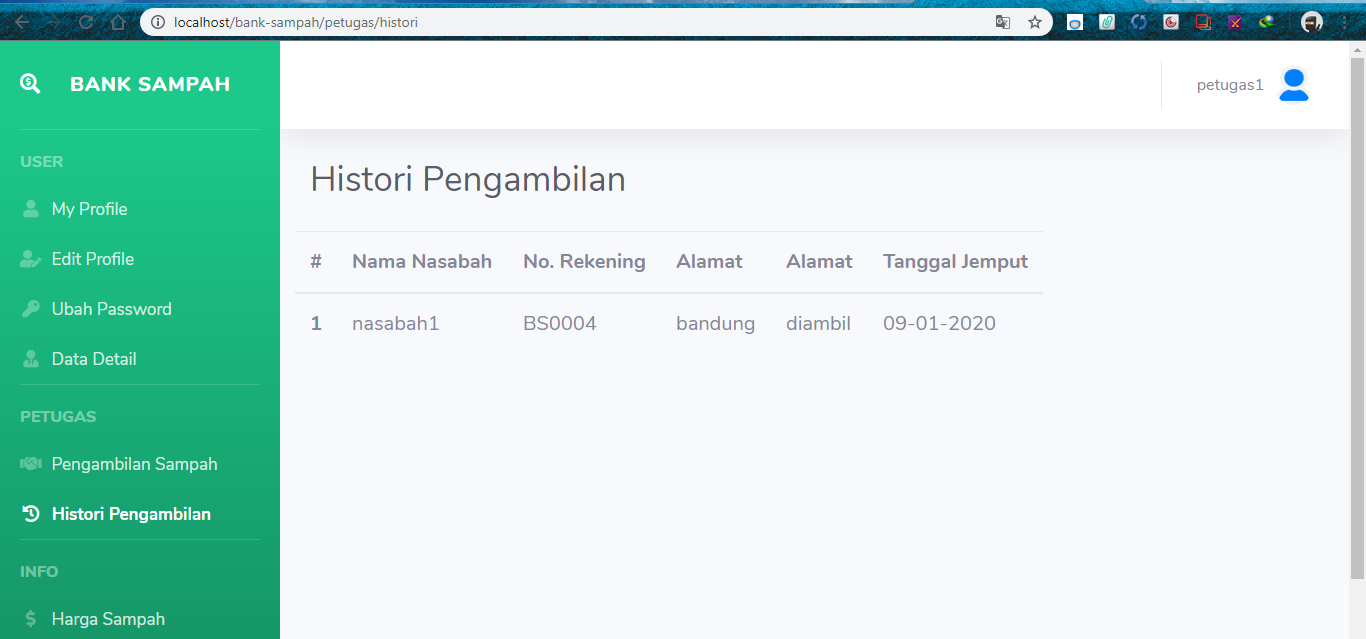
\includegraphics[width=8cm]{figures/analisis/31.png}
		\centering
		\caption{Gambar Page Histori Pengambilan}
	\end{figure}
Penjelasannya :
\begin{enumerate}
\item Pada halaman ini petugas akan mengecek aktivitas pengambilan sampah pada nasabah, sehingga petugas dapat mengetehaui nasabah dan tanggal berapa dia melakukan proses menabung smapah untuk dapat dilaporkan pada admin.
\item Jika proses penginputan berhasil maka akan muncul pada halaman histori pengambilan, bahwa sampah tersebut telah diambil.
\end{enumerate}	

\subsection{Tampilan Pada Android}
\subsubsection{Tampilan Page Home}
\hfill\\
	\begin{figure}[H]
		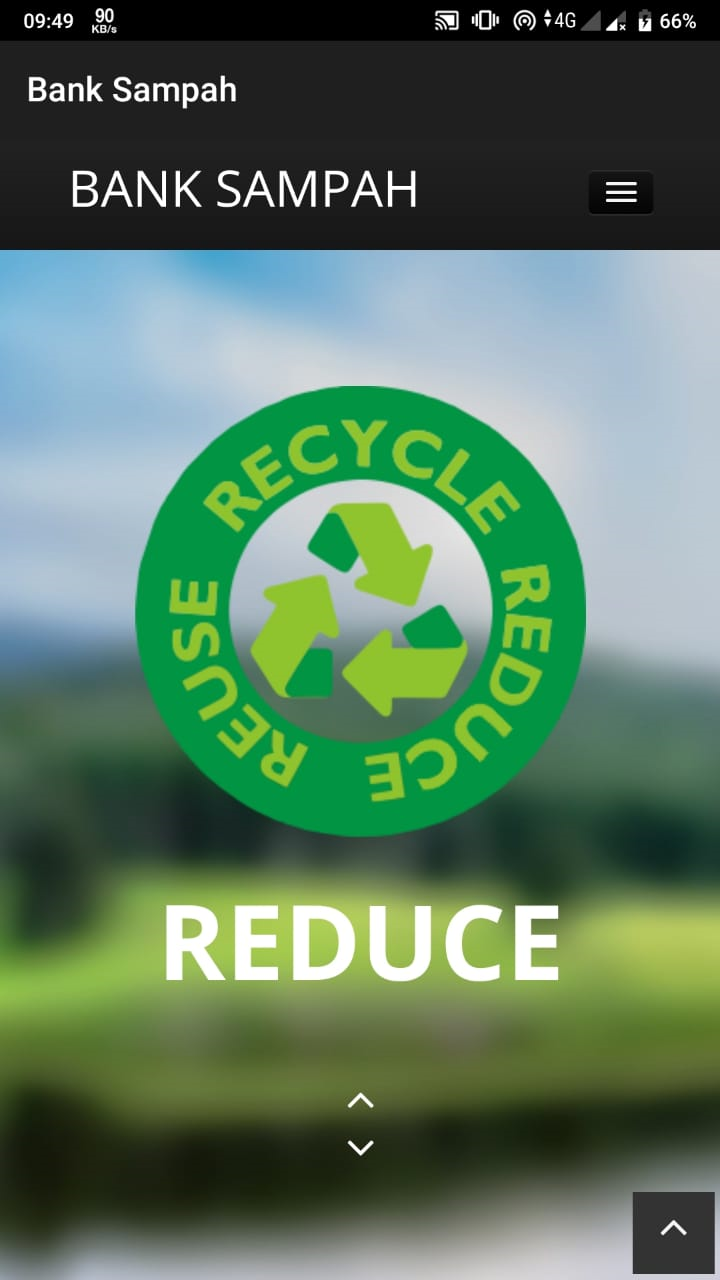
\includegraphics[width=8cm]{figures/analisis/32.png}
		\centering
		\caption{Gambar Page Home}
	\end{figure}
Penjelasannya :
\begin{enumerate}
\item Ketika user masuk ke aplikasi bank smapah user akan mmasuk ke Tampilan page awal tersebut.
\item Pada tamoilan awal ini user dapat melakukan proses login dan akan masuk ke halaman login.
\end{enumerate}

	\begin{figure}[H]
		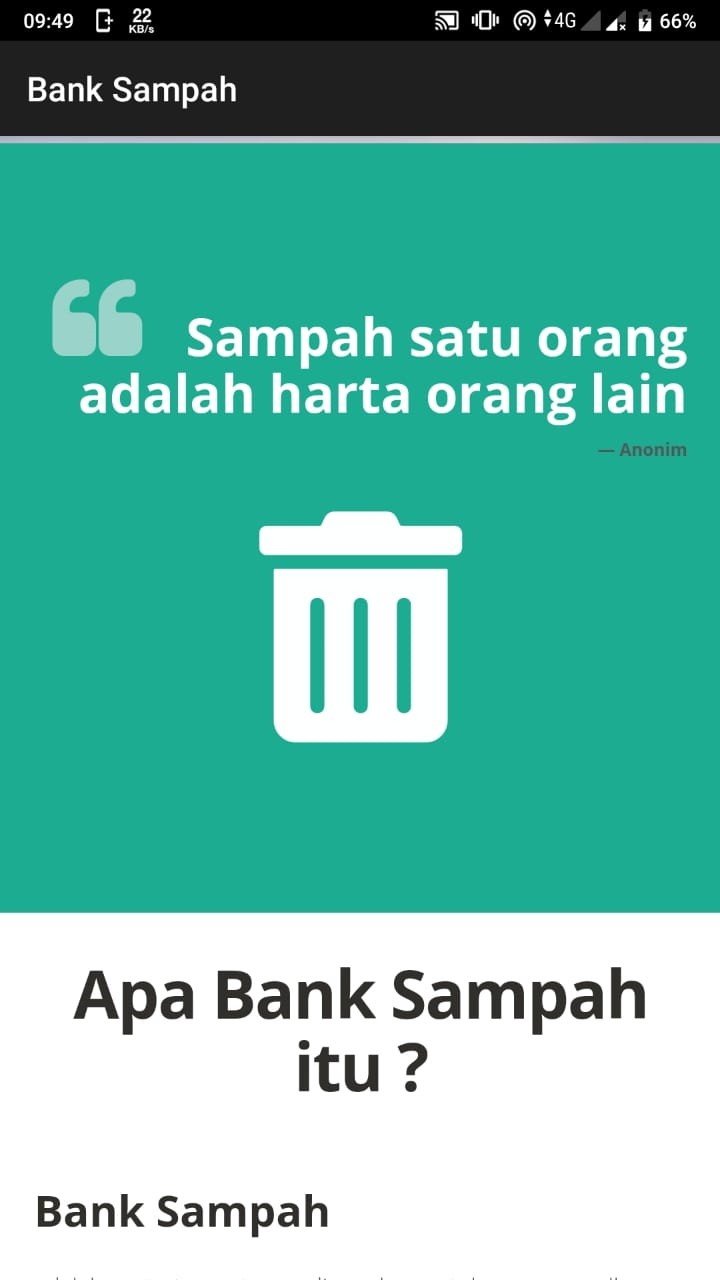
\includegraphics[width=8cm]{figures/analisis/33.png}
		\centering
		\caption{Gambar Page Home-2}
	\end{figure}
Penjelasannya :
\begin{enumerate}
\item Sebelum user melakukan proses login atau registrasi, user dapat melihat-lihat terlebih dahulu tampilan page awal ketika user masuk ke aplikasi bank sampah.
\end{enumerate}

	\begin{figure}[H]
		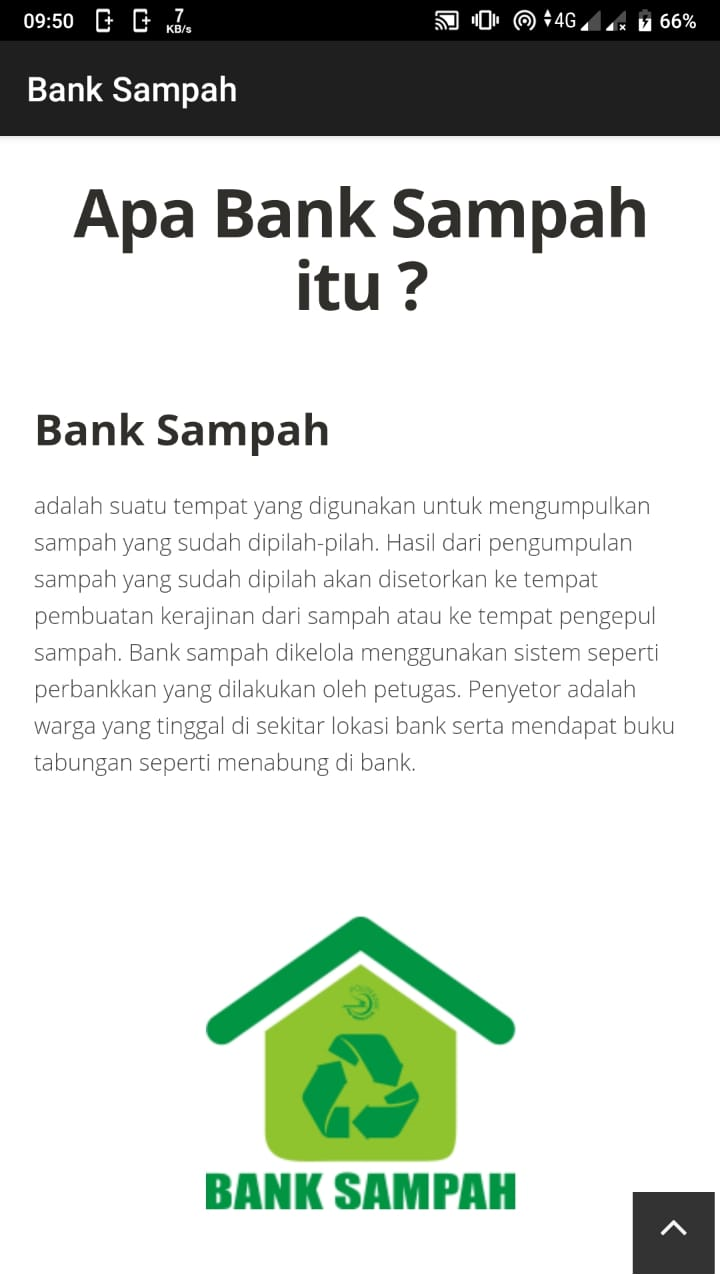
\includegraphics[width=8cm]{figures/analisis/34.png}
		\centering
		\caption{Gambar Page Home-3(Tentang)}
	\end{figure}
Penjelasannya :
\begin{enumerate}
\item Sebelum Pada  tampilan ini diberi penjelasan tentang pengertian bank sampah, agar masyarakat sekitar bisa lebih memahami betapa pentingnya bank sampah.
\end{enumerate}

\subsubsection{Tampilan Page Login}
\hfill\\
	\begin{figure}[H]
		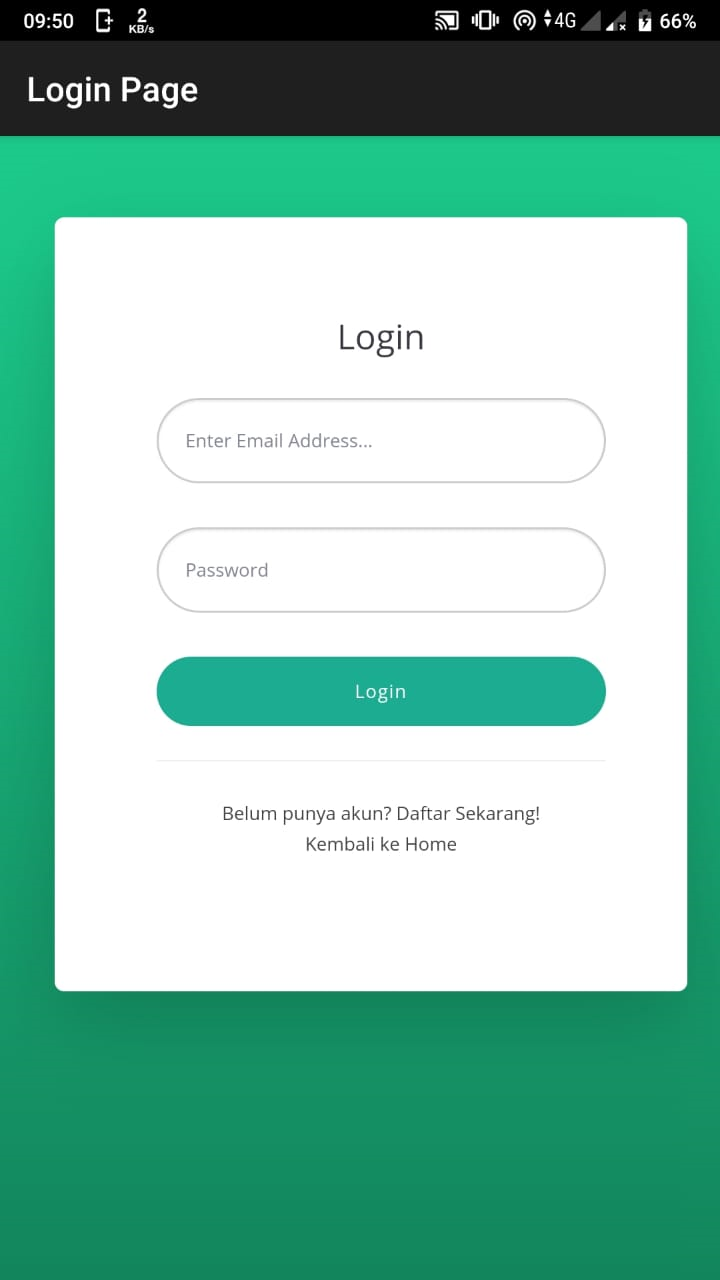
\includegraphics[width=8cm]{figures/analisis/35.png}
		\centering
		\caption{Gambar Page Login}
	\end{figure}
Penjelasannya :
\begin{enumerate}
\item Isikan Username dan Password kemudian klik Login.
\item Apabila proses login berhasil maka akan masuk ke form halaman utama yang sesuai dengan hak akses yang dimiliki.
\end{enumerate}

\subsubsection{Tampilan Page Profile}
\hfill\\
	\begin{figure}[H]
		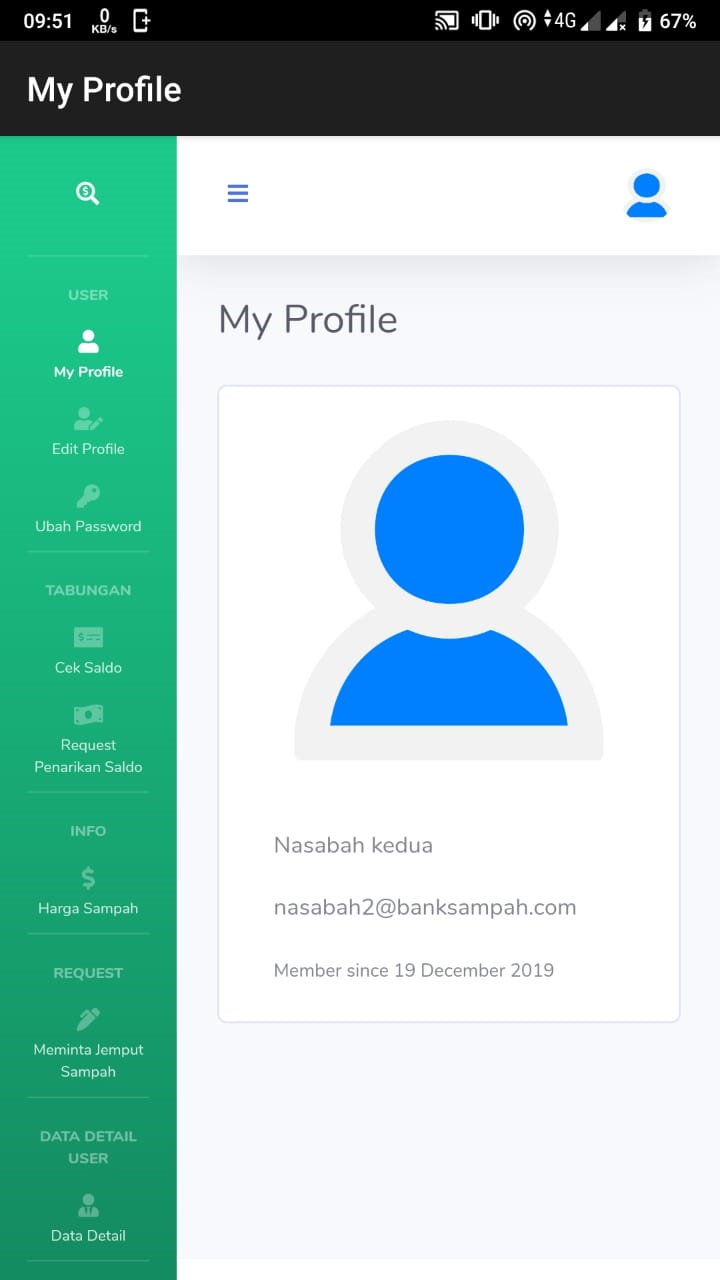
\includegraphics[width=8cm]{figures/analisis/36.png}
		\centering
		\caption{Gambar Page Profile}
	\end{figure}
Penjelasannya :
\begin{enumerate}
\item User dapat melakukan proses edit profile pada akun yang dimilikinya.
\item User dapat mengubah password sekaligus menambahkan foto profile.
\end{enumerate}

\subsubsection{Tampilan Page Tabungan}
\hfill\\
	\begin{figure}[H]
		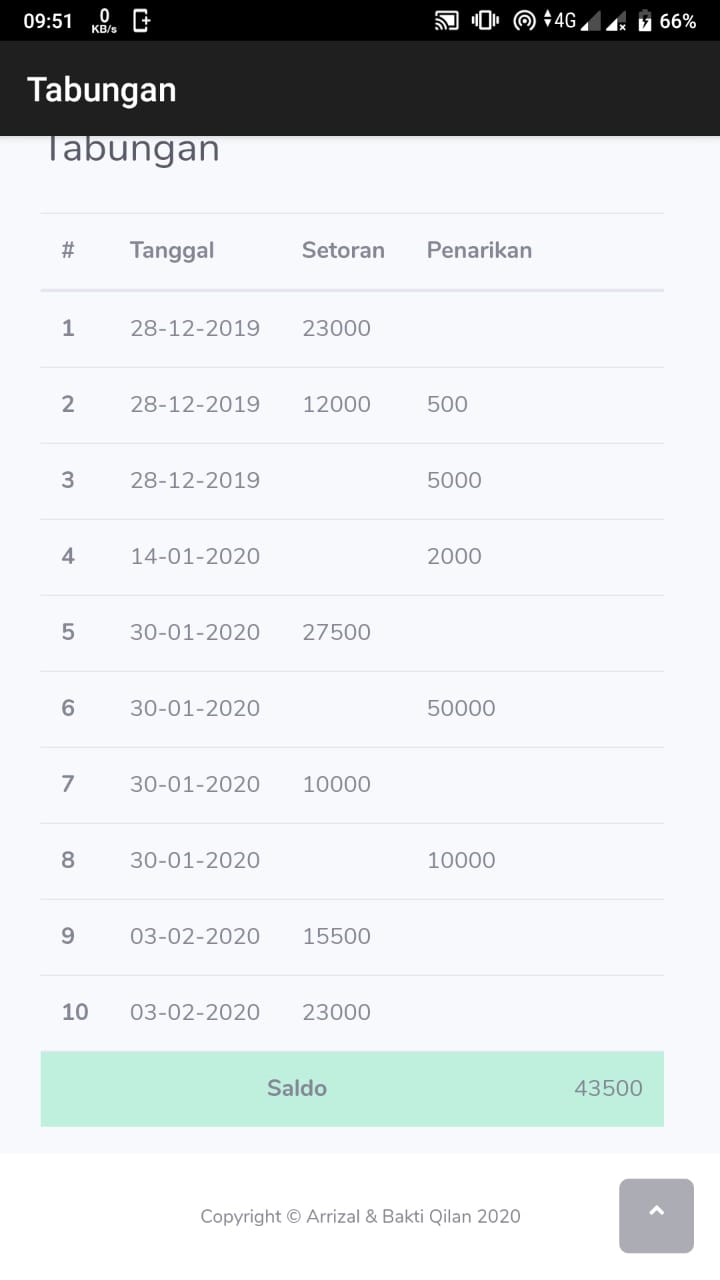
\includegraphics[width=8cm]{figures/analisis/37.png}
		\centering
		\caption{Gambar Page Tabungan}
	\end{figure}
Penjelasannya :
\begin{enumerate}
\item Ketika nasabah sudah di aktivasi oleh admin maka nasabah dapat melihat saldo sekaligus mendapatkan no.rekening.
\item Apabila nasabah sudah mendapatkan no rekening maka nasabah dapat melakukan proses menabung sampah.
\end{enumerate}